% EPL master thesis cover template
\documentclass{eplmastersthesis}

% Fill in here the information: title, student name, speciality, jury members
\title{Title of the master thesis}	% Master thesis title
\subtitle{Subtitle (optional)}			% Optional subtitle
\author{Firstname \textsc{Lastname}}	% Student name
\secondauthor{Firstname \textsc{Lastname}}	% Second student name if applicable
\speciality{Speciality}		% Speciality (use one of the following options):
										% Biomedical Engineering
										% Chemical and Materials Engineering
										% Civil Engineering
										% Computer Science
										% Computer Science and Engineering
										% Electrical Engineering
										% Electro-mechanical Engineering
										% Mathematical Engineering
										% Mechanical Engineering
										% Physical Engineering
%\options{Option(s)}		% If required by program commission mention options
\supervisor{Firstname \textsc{Lastname}}	% 1st supervisor name
\cosupervisor{Firstname \textsc{Lastname}}	% 2nd supervisor name if applicable
\readerone{Firstname \textsc{Lastname}}		% 1st reader name
\readertwo{Firstname \textsc{Lastname}}		% 2nd reader name
\readerthree{Firstname \textsc{Lastname}}	% 3rd reader name
\years{20..-20..}	% Academic year

\begin{document}

\maketitle					% To create front cover page
%\thispagestyle{empty}		% To suppress header and footer on the back of the cover page
\newpage\null\thispagestyle{empty}\newpage % Blank page

\pagestyle{fancy}

\pagenumbering{arabic}

\chapter{Results and discussion}
In this chapter, we will present the different results and discuss them.

\textcolor{red}{Expliquer ce qu'on va faire et tester}

\textcolor{red}{Mettre ici les trois "super mesh"}
\section{Multigrid}
In this section, we will test the coarse part of the preconditioner : the multigrid solver. This will be done in two steps. First, we will verify a well known property of the multigrid solvers : the h-independent convergence. We will also compare the number and iterations needed while varying key parameters of the model. Those tests will be performed on various meshes. The second part will focus on the influence of hanging nodes on the numerical solution. 

Let us before all present a type of numerical solution that can be obtained using the multigrid solver. Figure \ref{multi_simple_sol} shows an example of the numerical solution computed. We can see that even with $p=1$, we have a good approximation. This is because the forcing term is not at all oscillatory.

\begin{figure}
\centering
\includegraphics[scale=0.35]{Results/multi_simple_sol.eps}
\caption{Numerical solution using the multigrid solver of $\nabla^2 u = f$ for $f = -2\tanh(3x)\tanh(3y)(18-9\tanh^2(3x)-9\tanh^2(3y))$}
\label{multi_simple_sol}
\end{figure}

\subsection{H-independent convergence}
Let us first verify that our geometric multigrid solver has the required property and that the same number of iterations is needed to obtain a given accuracy, however small the elements. We will use the model problem throughout this section with the same right hand side. For all the tests below, the domain  will be : $\Omega = [-1;1]^2$. We will solve : 

\begin{align}
\nabla^2 u &= -\frac{\pi^2}{2}\cos(\frac{\pi}{2}x)\cos(\frac{\pi}{2}y) &\text{on $\Omega$} \\
u &= 0  &\text{on $\Gamma$}
\end{align}

It is easy to see that for the given domain, we have an analytic solution : 
$$u(x,y) = \cos(\frac{\pi}{2}x)\cos(\frac{\pi}{2}y))$$ 


Let us now explain how we define the error. We will look at the absolute difference between the value of the approximation and the value of the analytic solution at the global nodes and take the maximum. Formally, we have that the error after iteration $k$, $e_k$ is :

$$e_k = \max_i |u(x_i,y_i) - u_i^k|$$

Where $u_i^k$ is the value of our approximation at the global node $i$ after iteration $k$. Since $u_i^0 = 0$ for all $i$, it is clear that $e_0 = 1$.

Figure \ref{multi_mesh} shows the two "supra meshes" that we will refine during the tests. Some refinements will be uniform and some will be so that we have the presence of hanging nodes. We can note that even for the crooked mesh, the elements are not really distorted. It does not matter since we are only testing the h-independent convergence. Having a mesh with elements that are more distorted will only influence the accuracy of the approximation and not how the algorithm solve the linear system we want to solve. 

\begin{figure}
\centering
\begin{subfigure}{.5\textwidth}
  \centering
  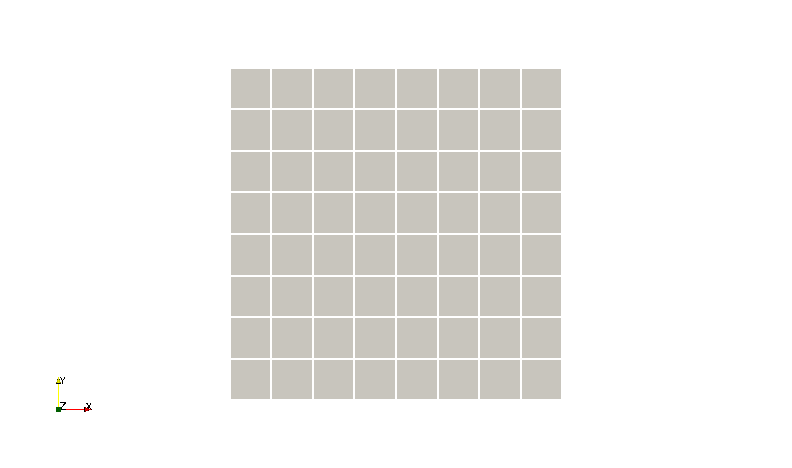
\includegraphics[width=1.2\linewidth]{Results/multi_mesh_1.png}
  \caption{Regular mesh}
  \label{multi_mesh_1}
\end{subfigure}%
\begin{subfigure}{.5\textwidth}
  \centering
  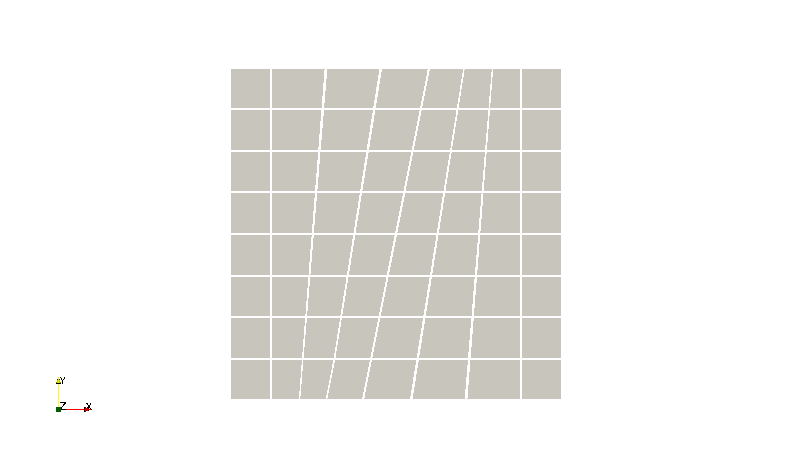
\includegraphics[width=1.2\linewidth]{Results/multi_mesh_2.png}
  \caption{Crooked mesh}
  \label{multi_mesh_2}
\end{subfigure}
\caption{The two "supra meshes" that will be refined during the tests for the multigrid solver. We have one regular mesh (left) where the elements are squares and one crooked mesh (right) where the elements are slightly distorted.}
\label{multi_mesh}
\end{figure}



Let us start with a simple V-cycle on the regular mesh (figure \ref{multi_mesh_1}) that we will refine uniformly. We will compare the errors when we increase the number of degrees of freedom and for different $\nu_1$ and $\nu_2$. The sum of the two smoothing parameters is chosen to be constant so that we have the same number of Jacobi iterations for all pairs $\nu_1$ and $\nu_2$. Here, we chose the sum to be equal to four.


\begin{table}
\centering
\begin{tabular}{c|ccccc}
\hline
 N & $2.6\:10^5$ & $1.1\:10^6$ & $4.2\: 10^6$& $1.7\:10^7$ & $6.7\:10^7$ \\
 \hline
  & $\nu_1=2$ & $\nu_2=2$ & & &\\
  \hline
  $e_1$ & 3.56e-02 & 3.56e-02 & 3.56e-02 & 3.56e-02 & 3.56e-02\\
  $e_2$ & 1.34e-03 &	1.34e-03 &	1.34e-03	& 1.34e-03	& 1.34e-03\\
  $e_3$ & 5.42e-05 &	5.66e-05 &	5.72e-05 &	5.73e-05 &	5.73e-05\\
  $e_4$ & 3.11e-06 &	2.90e-06 &	3.45e-06 &	3.59e-06 &	3.62e-06\\
  $e_5$ & 3.30e-06 &	9.48e-07 &	3.62e-07	& 3.50e-07 &	3.85e-07\\
  $e_6$ & 3.17e-06 &	8.14e-07 &	2.26e-07 &	8.26e-08 &	5.23e-08\\
  \hline
  & $\nu_1=3$ & $\nu_2=1$ & & &\\
  \hline
  $e_1$ & 3.70e-02 &	3.71e-02 &	3.71e-02 &	3.71e-02 &	3.71e-02\\
  $e_2$ & 1.62e-03 &	1.63e-03 &	1.63e-03 &	1.63e-03 &	1.63e-03\\
  $e_3$ & 1.04e-04 &	1.06e-04 &	1.07e-04 &	1.07e-04	& 1.07e-04\\
  $e_4$ & 1.10e-05 &	1.22e-05 &	1.27e-05 &	1.29e-05 & 	1.29e-05\\
  $e_5$ & 4.47e-06 &	2.20e-06 &	1.96e-06 &	2.10e-06 & 	2.13e-06\\
  $e_6$ & 3.34e-06 &	1.00e-06 &	4.38e-07 &	3.53e-07 &	3.88e-07\\
  \hline
  & $\nu_1=1$ & $\nu_2=3$ & & &\\
  \hline
  $e_1$ & 3.57e-02 &	3.57e-02 &	3.57e-02 &	3.57e-02 &	3.57e-02\\
  $e_2$ & 1.29e-03 &	1.29e-03 &	1.29e-03 &	1.29e-03 &	1.29e-03\\
  $e_3$ & 4.66e-05 &	4.89e-05 &	4.95e-05 &	4.96e-05 &	4.97e-05\\
  $e_4$ & 1.53e-06 &	1.53e-06 &	2.10e-06 &	2.24e-06 &	2.28e-06\\
  $e_5$ & 3.08e-06 &	7.31e-07 &	1.43e-07 &	1.17e-07 &	1.51e-07\\
  $e_6$ & 3.14e-06 &	7.83e-07 &	1.95e-07 &	4.80e-08 &	1.13e-08\\
  \hline
   & $\nu_1=4$ & $\nu_2=0$ & & &\\
  \hline
  $e_1$ & 4.55e-02 &	4.55e-02 &	4.55e-02 &	4.55e-02 &	4.55e-02\\
  $e_2$ & 3.26e-03 &	3.26e-03 &	3.26e-03 &	3.26e-03 &	3.26e-03\\
  $e_3$ & 4.64e-04 &	4.71e-04 &	4.71e-04 &	4.71e-04 &	4.71e-04\\
  $e_4$ & 9.24e-05 &	9.60e-05 &	9.65e-05 &	9.67e-05 &	9.67e-05\\
  $e_5$ & 1.74e-05 &	2.04e-05 &	2.12e-05 &	2.14e-05 &	2.14e-05\\
  $e_6$ & 6.17e-06 &	3.86e-06	& 4.55e-06	& 4.74e-06 &	4.78e-06\\
  \hline
  & $\nu_1=0$ & $\nu_2=4$ & & &\\
  \hline
  $e_1$ & 3.58e-02 &	3.58e-02 &	3.58e-02 &	3.58e-02 &	3.58e-02\\
  $e_2$ & 1.29e-03 &	1.29e-03 &	1.29e-03 &	1.29e-03 &	1.29e-03\\
  $e_3$ & 4.53e-05 &	4.77e-05 &	4.82e-05 &	4.84e-05 &	4.84e-05\\
  $e_4$ & 1.17e-06 &	1.31e-06 &	1.89e-06 &	2.03e-06 &	2.07e-06\\
  $e_5$ & 3.03e-06 &	6.80e-07 &	9.14e-08 &	7.66e-08 &	1.12e-07\\
  $e_6$ & 3.13e-06 &	7.76e-07 &	1.87e-07 &	4.04e-08 &	3.62e-09\\
  \hline
\end{tabular}
\caption{Errors after $k$ iterations of a V-cycle ($e_k$) for the regular mesh uniformly refined to have $N$ degrees of freedom and for different values of the parameters $\nu_1$ and $\nu_2$}
\label{multi_err_nu}
\end{table}

The results are shown in table \ref{multi_err_nu}. We can see that we indeed have an h-independent convergence of the solver. For every pair of the smoothing parameters, at least for the first few iterations, the error $e_k$ is identical for all values of $N$. Except for the pair $\nu_1 = 4$ and $\nu_2 = 0$, each iteration roughly decrease the error by one decimal point.

We can also note that the values of the parameters influence the convergence. For this particular problem and this particular mesh, the values $\nu_1 = 0$ and  $\nu_2 = 4$ seem to be the best as the error is smaller after the same number of iterations than for the other pairs. The less post smoothing iterations ($\nu_2$) we do, the slower the convergence. This is true for $\nu_2 = 1$ where the error on the finest mesh after six iterations is a hundred times larger than on the same mesh after the same number of iterations for $\nu_2=4$, and it is clearer still for $\nu_2=0$ where the error is a thousand times larger after six iterations on the finest mesh.

We have to note that even tough the errors are identical for all meshes at first, we have a difference after a few iterations. This can be explained by the fact that our geometric multigrid algorithm actually solves a linear system whereas the error is measured as the difference between the analytic solution and the solution of the linear system. Thus, even if we solved the linear system exactly, we would still have an error and that error should decrease as the number of degrees of freedom increases. This is indeed what we observe here. For example, for the mesh with $N=2.6\:10^5$, we can see that after six iterations, we have almost converged and that the error stays around $3.14\:10^{-6}$. Even if we did several more iterations, the error would not decrease significantly. That is because we have the solution of the linear system and the error is only due to the discretization. If we refine the mesh and go to $N=6.7\:10^7$, then we can get smaller errors (of the order of $10^{-8}$).

Let us now explore the results for the crooked mesh (figure \ref{multi_mesh_2}). Here also, we should expect an h-independent convergence. We only show the results for $\nu_1=2$ and $\nu_2=2$ but the same commentary applies for the other pairs. The results can be seen on table \ref{multi_err_crook}

\begin{table}
\centering
\begin{tabular}{c|ccccc}
\hline
N & $2.6\:10^5$ & $1.1\:10^6$ & $4.2\: 10^6$& $1.7\:10^7$ & $6.7\:10^7$ \\
 \hline
  & $\nu_1=2$ & $\nu_2=2$ & & &\\
  \hline
  $e_1$ & 3.64e-02 &	3.64e-02 &	3.64e-02 &	3.64e-02 &	3.64e-02\\
  $e_2$ & 2.56e-03 &	2.49e-03 &	2.46e-03	& 2.44e-03 &	2.43e-03\\
  $e_3$ & 7.41e-04 &	6.33e-04 &	5.80e-04 &	5.54e-04 &	5.41e-04\\
  $e_4$ & 6.15e-04 &	3.15e-04 &	1.62e-04 &	1.35e-04 &	1.28e-04\\
  $e_5$ & 5.96e-04 &	3.01e-04 &	1.52e-04 &	7.67e-05	& 4.76e-05\\
  $e_6$ & 5.91e-04 &	2.98e-04 &	1.50e-04 &	7.50e-05 &	3.77e-05\\
  \hline
\end{tabular}
\caption{Errors after $k$ iterations of a V-cycle ($e_k$) for the crooked mesh uniformly refined to have $N$ degrees of freedom and for $\nu_1=2$ and $\nu_2=2$}
\label{multi_err_crook}
\end{table}

We can see that the for the first few iterations, the error $e_k$ is independent of the mesh. However, the note we made earlier is much clearer here. Because the mesh is not regular, the effect of discretization are more important and therefore we will not reach the same accuracy than we did before. That is why after six iterations, the less refined grid ($N = 2.6\:10^5$) still has an error of $5.91\:10^{-4}$. More iterations will not have a great impact on the solution since the error is mostly due to the discretization.

\subsection{Influence of hanging nodes}
We will now investigate the influence of hanging nodes on our solution. We will present the results only for the regular mesh but the tests have been performed on both and the same conclusions apply to the crooked mesh.

We will compare the values of the error between one mesh with no hanging nodes, one where we only have refined the lower left part of the domain once, and one where we have a rapid transition between two parts  of different refinement level (which will occur often in AMR).

Figure \ref{multi_mesh_hanging} presents the latter two meshes. For the mesh in figure \ref{multi_mesh_hanging_2}, we have refined thrice more in a certain region than in the adjacent one. Since we do not allow adjacent quadrants to be more than one level apart, we obtain a "layer" where the levels of the quadrants is rapidly changing. In order to compare solutions, we made sure that the largest quadrants in all three meshes had the same size. This means that the meshes with hanging nodes have a lot more degrees of freedom.  

\begin{figure}
\centering
\begin{subfigure}{.5\textwidth}
  \centering
  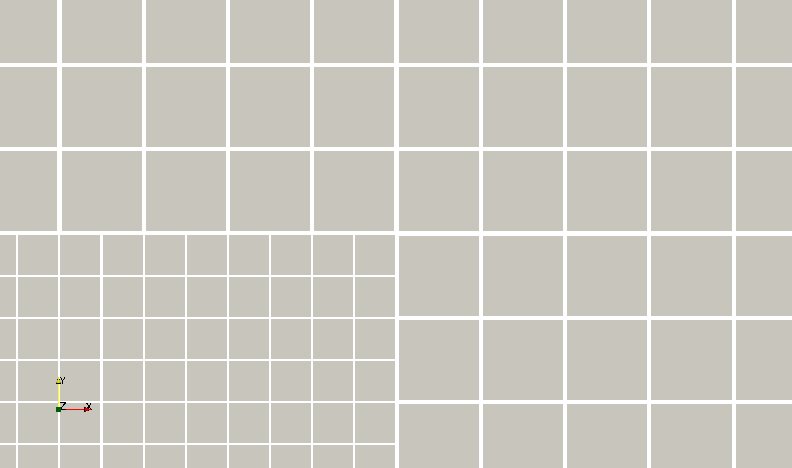
\includegraphics[width=0.8\linewidth]{Results/multi_mesh_hanging_1.png}
  \caption{Two levels}
  \label{multi_mesh_hanging_1}
\end{subfigure}%
\begin{subfigure}{.5\textwidth}
  \centering
  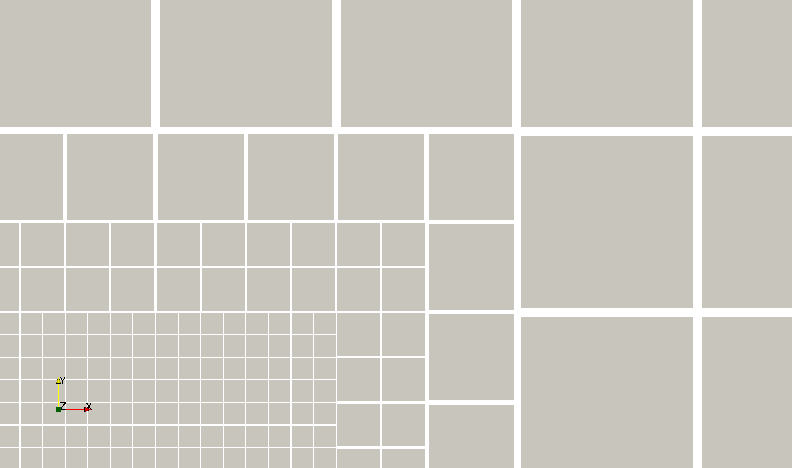
\includegraphics[width=0.8\linewidth]{Results/multi_mesh_hanging_2.png}
  \caption{Levels rapidly changing}
  \label{multi_mesh_hanging_2}
\end{subfigure}
\caption{Zoom on a certain part of the two meshes containing hanging nodes that will be used to test the multigrid solver. We have one mesh where we only have refined a part of the domain once more than the rest (left) and a mesh where we have refined a part thrice more than the rest which results in levels changing rapidly (right).}
\label{multi_mesh_hanging}
\end{figure}


\begin{table}
\centering
\begin{tabular}{c|ccc}
\hline
Meshes & No hanging nodes & Figure \ref{multi_mesh_hanging_1} & Figure \ref{multi_mesh_hanging_2}\\
\hline
N & $4.2\:10^6$ & $7.3\:10^6$ & $7.0\: 10^7$ \\
  \hline
  $e_1$ & 3.56e-02 &	3.56e-02 &	3.56e-02 \\
  $e_2$ & 1.34e-03 &	1.34e-03 &	1.34e-03	\\
  $e_3$ & 5.72e-05 &	5.72e-05 &	5.74e-05 \\
  $e_4$ & 3.45e-06 &	3.47e-06 &	3.64e-06 \\
  \hline
\end{tabular}
\caption{Errors after $k$ iterations of a V-cycle ($e_k$) for a mesh without hanging nodes and the two meshes presented in figure \ref{multi_mesh_hanging}. Each mesh has $N$ degrees of freedom and the smoothing parameters were $\nu_1 = 2$ and $\nu_2 =2$.}
\label{multi_err_hanging}
\end{table}

Table \ref{multi_err_hanging} shows the results for the three different meshes using a V-cycle and with the smoothing parameters  $\nu_1=2$ and $\nu_2 = 2$. Here again, we can see that the convergence is h-independent and that one iteration gives us roughly one more decimal. The presence of hanging nodes has no influence on the error we observe after a given number of iterations. The same result is observed with all pairs of the smoothing parameters and with other meshes.

This will be important in the next sections when we will use our multigrid solver as a preconditioner. Indeed, we will see that it is the coarse correction that allow for h-independent convergence.  


 




\section{Fine preconditioner}
Let us now move on to the fine part of the preconditioner : the overlapping additive Schwarz preconditioner. We will test it by using the preconditioned conjugate gradients method described earlier but, for now, the preconditioner will only consist of the fine part (i.e. $P = P^f$).

As in the previous section, we will perform the tests in two parts : first, we will use meshes with elements that are distorted or not but with no hanging nodes. Then, we will see how the fine preconditioner performs in the presence of hanging nodes also for meshes that are distorted or not. Here, of course, we will use interpolations of higher degree. Typically, the tests will be performed for $p=2,4,6,8$.

\subsection{No hanging nodes}

Let us first present the problem we will use throughout this section. The forcing term will be chosen more oscillatory than in the previous part since we use interpolations of higher degree. As before, the domain is : $\Omega = [-1;1]^2$ and $\Gamma$ is the boundary. The problem is : 

\begin{align}
\nabla^2 u &= -8\pi^2\sin(2\pi x)\sin(2\pi y) &\text{on $\Omega$} \label{eq:prob2}\\
u &= 0  &\text{on $\Gamma$}
\end{align}

This problem has an analytic solution and it is easy to convince oneself that this solution is given by : 

$$ u(x,y) = \sin(2\pi x)\sin(2\pi y)$$

\begin{figure}
\centering
\includegraphics[scale=0.35]{Results/fine_simple_sol.eps}
\caption{Numerical solution to problem \ref{eq:prob2} using an interpolation of order $p=2$ and $1.0\:10^6$ degrees of freedom on a regular mesh with no hanging nodes.}
\label{fine_simple_sol}
\end{figure}

Figure \ref{fine_simple_sol} shows the numerical solution to the problem above for $p=2$ and $1.0\:10^6$ degrees of freedom for a regular mesh. We can note that it is exactly the same number of degrees of freedom as if we had refined uniformly once more and used an interpolation of degree $p=1$. Let us then compare how the two approximations perform. We solved the problem for $p=1$ with our multigrid solver and the problem for $p=2$ with the PCG and the fine preconditioner. Let us denote $u^j_i$ as the value of the approximation for $p=j$ at node $i$. We have that : 

\begin{align*}
e^1 &= \max_i |u^1_i - u(x_i,y_i)| = 5.02\: 10^{-5}\\
e^2 & = \max_i |u^2_i - u(x_i,y_i)| = 1.01 \: 10^{-9}
\end{align*}

We can see that with the same number of degrees of freedom, an approximation using $p=2$ is much more accurate. This is because the solution is really smooth and is better approximated using a higher order interpolation than a bilinear interpolation on smaller quadrants. This is one example of the reasons we want to use higher order interpolations. 

\subsubsection{Regular meshes}

Let us now move on to the comparison for different degrees of the number of iteration needed to reach a given accuracy as a function of the number of quadrants. We will take our regular mesh and uniformly refine it. Then, for $p=2,4,6,8$, we will see how many iterations are needed to reach a given error on the norm of the residual. Let us denote $r_k$ the residual after iteration $k$ of the preconditioned conjugate gradients. Of course, since our initial guess is zero, we have that $r_0 = b$ (since we are solving the linear system $Au = b$). For the following tests, our stopping criterion is given by :

$$ \frac{||r_k||_2}{||r_0||_2} < 10^{-3}$$

Figure \ref{fine_reg_iter} shows the results. To put the data in perspective, we also have to show the number of degrees of freedom. Indeed, for a given number of quadrants, the higher degree the interpolation is, the more nodes we have. Table \ref{fine_reg_table} contains the number of nodes for each mesh and for each degree $p$.

\begin{table}
\centering
\begin{tabular}{c|ccccc}
\hline
Number of quadrants & $16^2$ & $32^2$ & $64^2$ & $128^2$ & $256^2$\\
\hline
$p=2$ & $1.1\:10^3$ & $4.2\:10^3$ & $1.7\:10^4$ & $6.6\:10^4$ & $2.6\:10^5$\\
$p=4$ & $4.2\:10^3$ & $1.7\:10^4$ & $6.6\:10^4$ & $2.6\:10^5$ & $1.1\:10^6$\\
$p=6$ & $9.4\:10^3$ & $3.7\:10^4$ & $1.5\:10^5$ & $5.9\:10^5$ & $2.4\:10^6$\\
$p=8$ & $1.7\:10^4$ & $6.6\:10^4$ & $2.6\:10^5$ & $1.1\:10^6$ & $4.2\:10^6$\\
\hline
\end{tabular}
\caption{Number of degrees of freedom for a regular mesh with different number of quadrants and for different degrees of interpolation.}
\label{fine_reg_table}
\end{table}

\begin{figure}
\centering
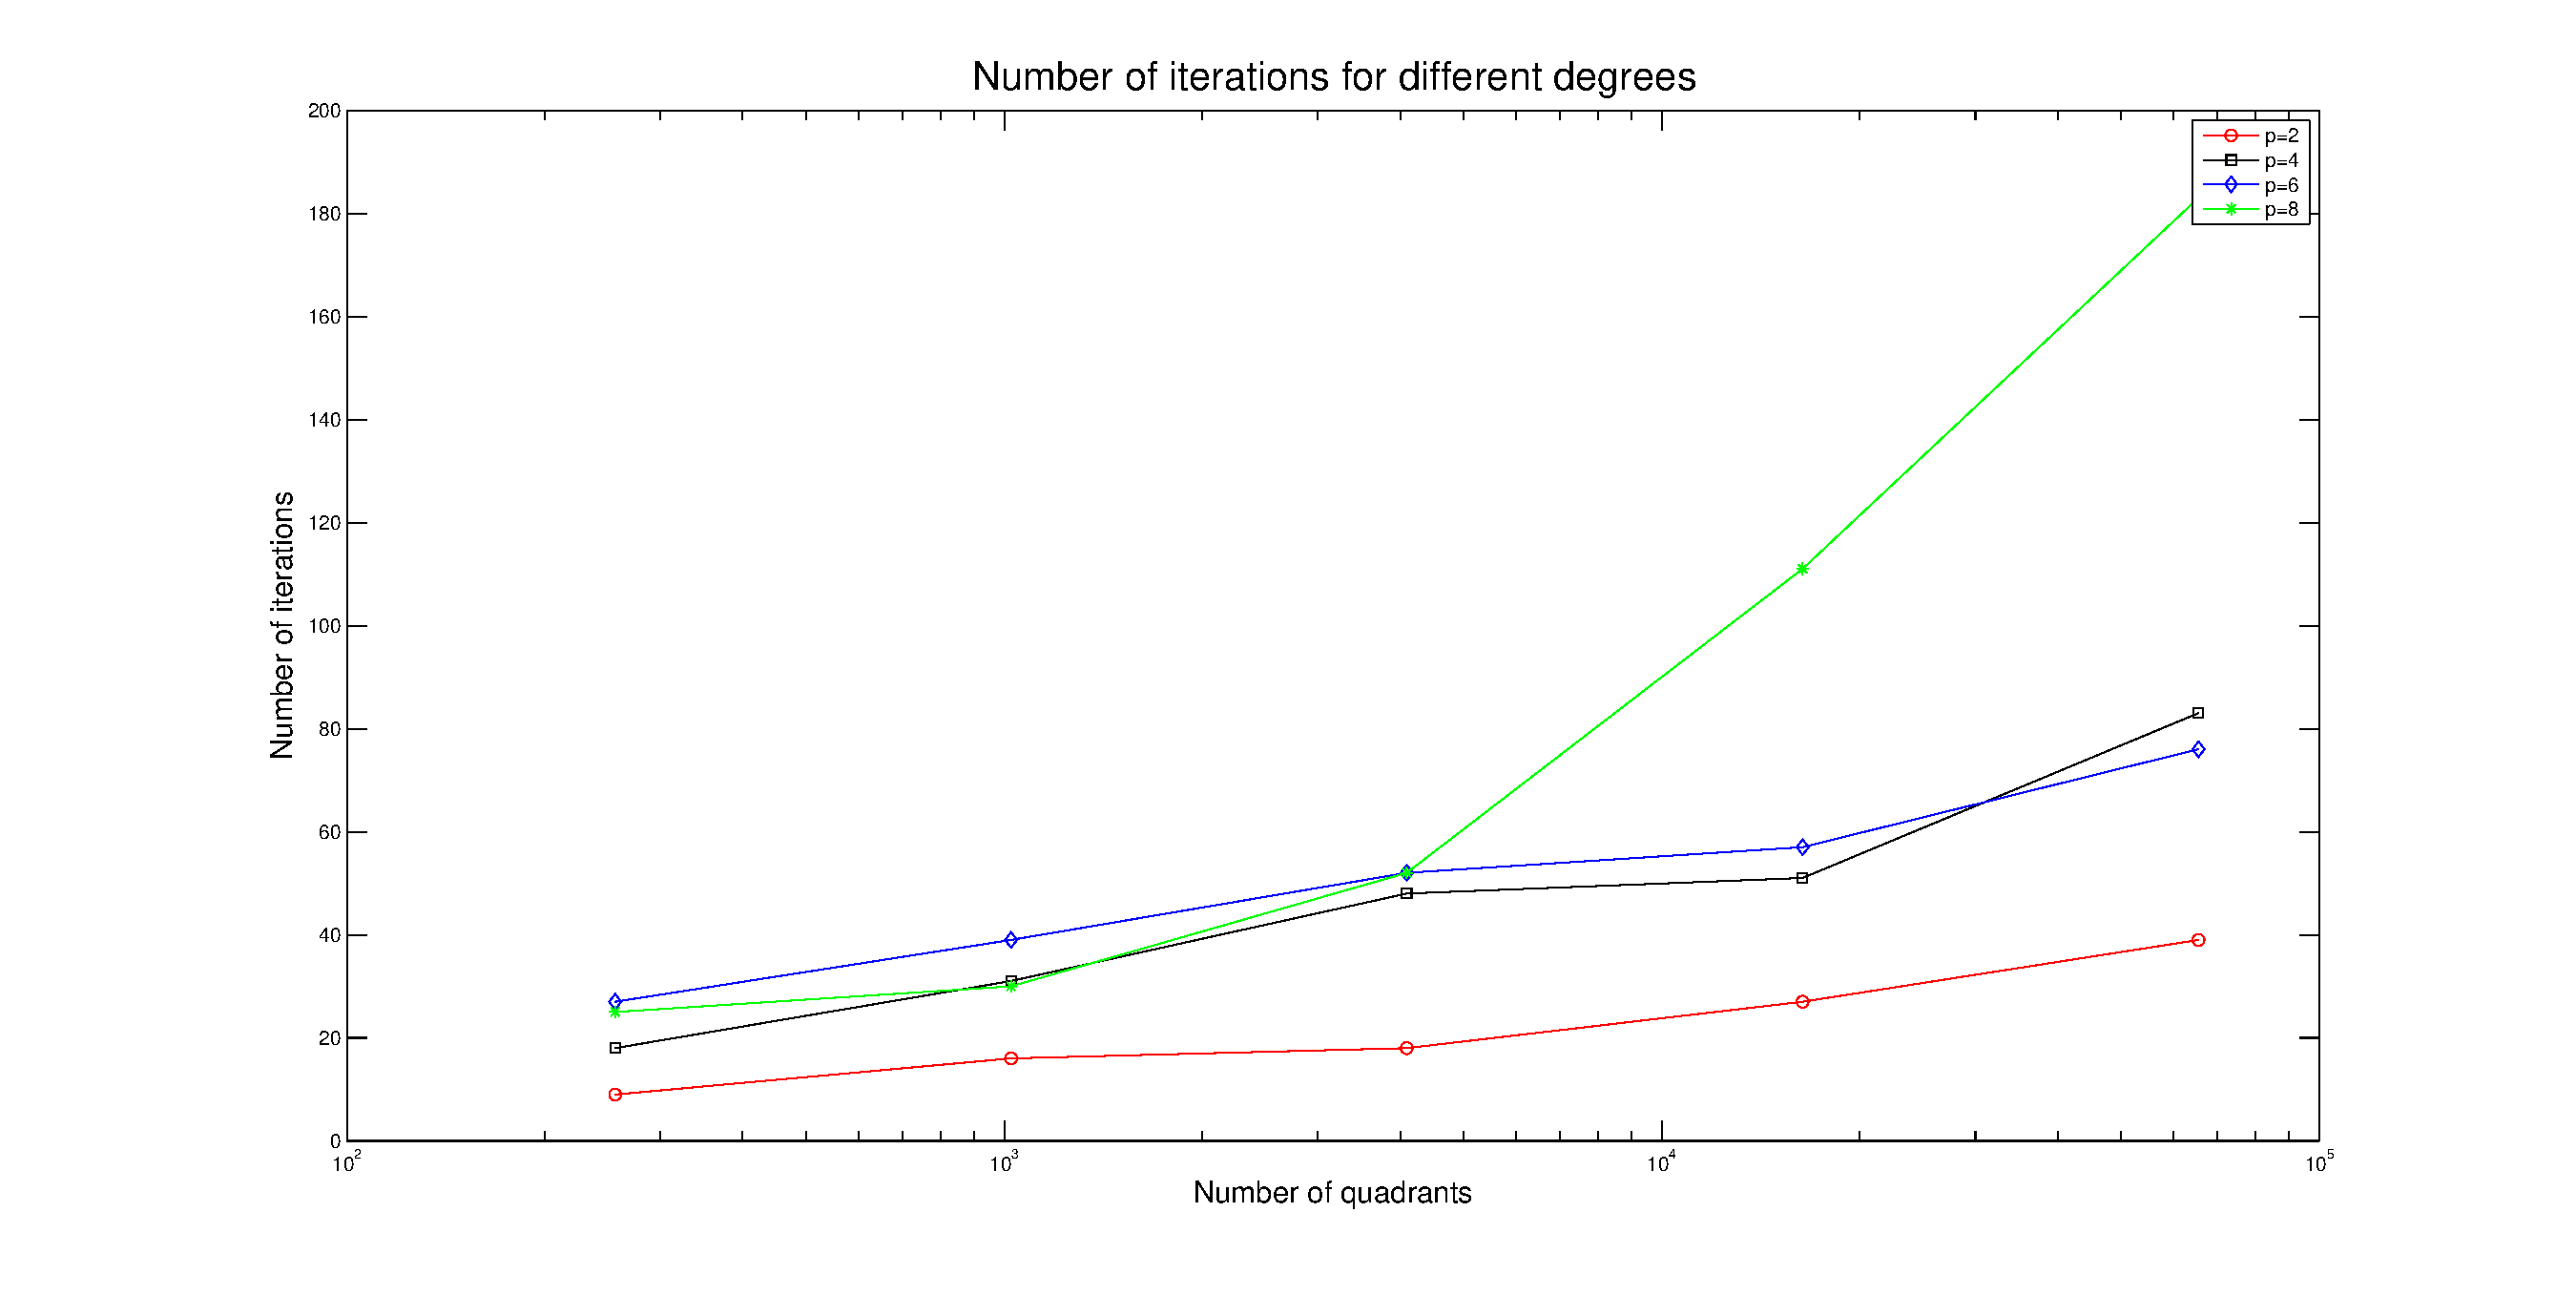
\includegraphics[scale=0.35]{Results/fine_reg_iter.eps}
\caption{Number of iterations of PCG with only the fine preconditioner for different degree $p$ of interpolation as a function of the number of quadrants in a regular mesh.}
\label{fine_reg_iter} 
\end{figure}

We can see that, even without the coarse preconditioner, we are solving the system in a small number of iterations compared to the number of degrees of freedom. For example, we only do about 80 iterations to solve the system with $2.4\: 10^{6}$ degrees of freedom and with interpolations of degree $p=6$. 

 We can also see that for every degree, the number of iterations increases when we refine the mesh. This is to be expected since the information from the boundaries has to go through more quadrant before propagate to the entire domain. Asymptotically, the number of iterations is expected to double as the number of quadrants is multiplied by four (i.e. the mesh size is divided by two). We can see that it is not yet the case here.

A last remark we can make is that the number of iterations tends to increase when the degree of the interpolation increases. This is especially true for the finest mesh where we need 183 iterations for $p=8$ where we only need 39 iterations for $p=2$. This can be explained by the fact that the size of the overlap decreases when $p$ grows. As mentioned in \textcolor{red}{Ref here!!}, this issue would be fixed if we imposed a constant overlap.

\subsubsection{Meshes with distorted elements}
Let us now move on to meshes that are not regular anymore. Let us remember that when we developed the fine preconditioner, we assumed that the elements were rectangular which allowed us to compute the analytic solution to the problem. This part explores the influence of having distorted elements on the number of iterations needed to obtain a given accuracy. 

\begin{figure}
\centering
\begin{subfigure}{.5\textwidth}
  \centering
  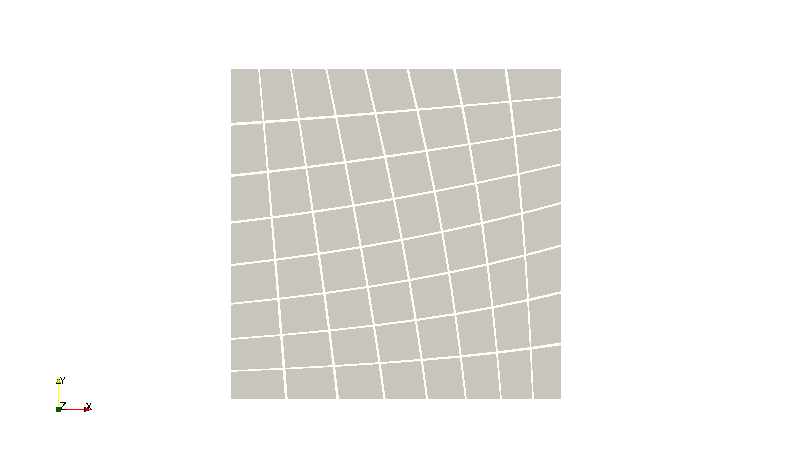
\includegraphics[width=1.2\linewidth]{Results/fine_mesh_deform_1.png}
  \caption{Mesh with $a=1.1$}
  \label{fine_mesh_deform_1}
\end{subfigure}%
\begin{subfigure}{.5\textwidth}
  \centering
  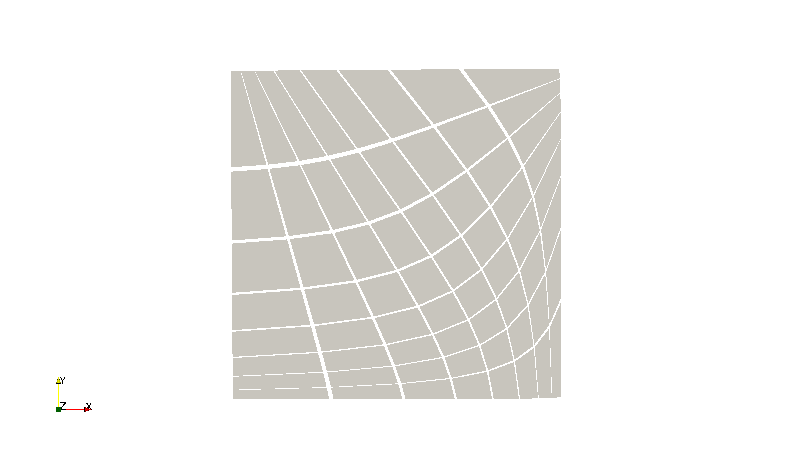
\includegraphics[width=1.2\linewidth]{Results/fine_mesh_deform_2.png}
  \caption{Mesh with $a=1.4$}
  \label{fine_mesh_deform_2}
\end{subfigure}
\caption{Examples of the meshes used for the tests of the fine preconditioner with distorted elements. The meshes are created using GMSH with its progression tool. The key parameter is the common ratio $a$ that we will be increasing progressively.}
\label{fine_mesh_deform}
\end{figure}

To control the deformation, we will continually deform the regular mesh using the progression tool of GMSH \textcolor{red}{ref here!!}. The deformation is performed using a geometric progression, using the common ratio $a$ as the parameter. Obviously, the higher the parameter $a$, the more distorted the mesh is. It is clear that for $a=1$, we have a regular mesh. Figure \ref{fine_mesh_deform} presents three meshes of obtained with the progression with GMSH. On the left we used $a = 1.1$ and on the right we used $a=1.4$. 

Using the same tolerance as in the previous part, we ran the preconditioned conjugate gradients with the fine preconditioner for those new meshes. The order of the interpolation used is $p=2$. The results are given in figure \ref{fine_dist_iter}.

We can see, as it was expected, that the more we deform the mesh, the more iterations we need to do in order to obtain the wanted accuracy. The fact that, for distorted elements, we do not invert exactly the system but use an approximation allows us to compute the fine preconditioner efficiently even when we have a lot of elements but we can see here that it also costs more iterations of the preconditioned conjugate gradients. However, the gain is still huge. Indeed, for a degree of interpolation $p$, we have $(p+3)^2$ nodes per overlapping subdomain. This means a complexity of $\mathcal{O}((p+3)^6)$ to solve the system exactly. Instead, with the method we use, the only need to do a few matrix multiplications where the matrices have $(p+3)$ rows and columns. This means a complexity of $\mathcal{O}((p+3)^2)$. Even with $p=2$, the results shows that it is much faster to not take geometric factors into account. 

We can also note that the effect of increasing the number of elements (i.e. reducing the mesh size) on the number of iterations is clearer here. For example, for the mesh with $a = 1.15$, we need 10 iterations for $8^2$ elements, 18 iterations for $16^2$ elements and 39 iterations for $32^2$ elements. The same explanation applies here : when we multiply the number of elements by four, we roughly multiply the number of quadrants in each direction by two and therefore the information needs twice as many iterations to propagate to the domain. 

\begin{figure}
\centering
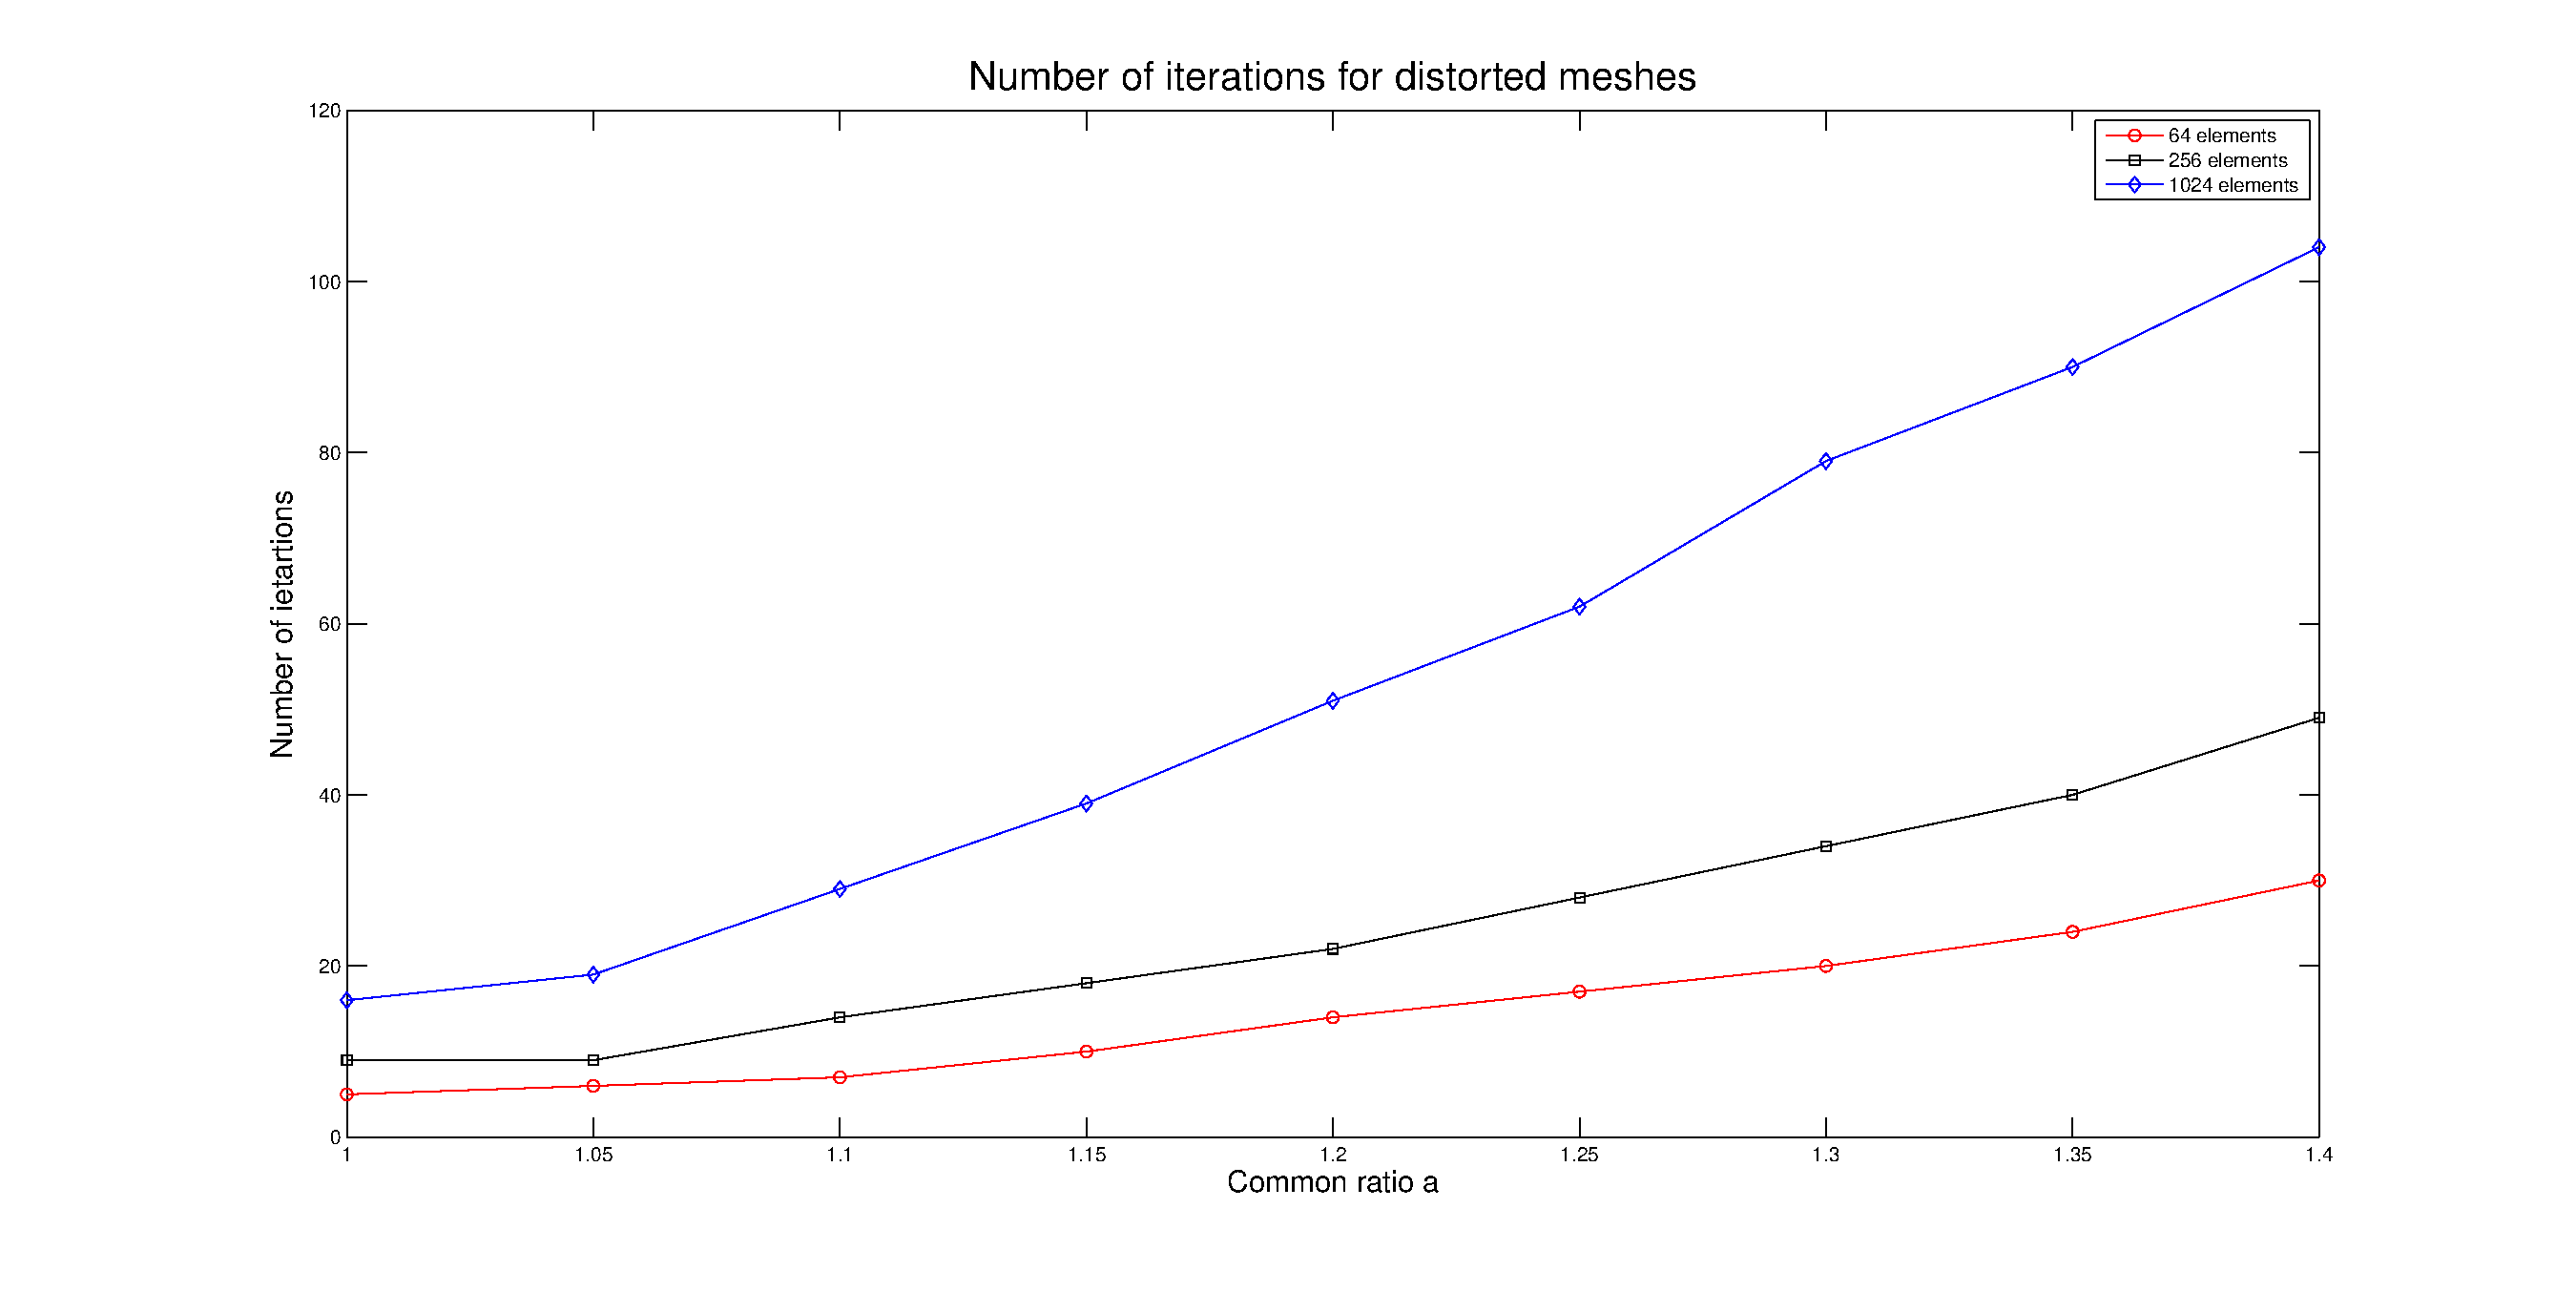
\includegraphics[scale=0.35]{Results/fine_dist_iter.eps}
\caption{bla}
\label{fine_dist_iter}
\end{figure}



\subsection{Influence of hanging nodes}
 In this part, we will explore the influence of hanging nodes on the number of iterations needed by the preconditioned conjugate gradients with the fine preconditioner to converge. Because we want meshes that are not artificial and come from real AMR applications, we will change the forcing term in this part and we will also use a recursive refine function when we build the mesh with p4est. 
 
 Let us first define the problem and the forcing term. As before, the domain is : $\Omega = [-1;1]^2$ and $\Gamma$ is the boundary. We will solve : 
 
 \begin{align}
 \nabla^2 u &= -2\tanh(nx)\tanh(my)\left[ n^2(1-\tanh(nx)^2) + m^2(1-\tanh(my)^2)\right] &\text{on $\Omega$} \label{eq:prob3}\\
u &= \tanh(nx)\tanh(my)  &\text{on $\Gamma$}
 \end{align}
 
 We can see that problem \ref{eq:prob3} has an analytic solution that is given by :
 
 $$u(x,y) = \tanh(nx)\tanh(my)$$
 
 The parameters $n$ and $m$ can be adjusted to make the jump in the hyperbolic tangent more steep. An example of a numerical solution with $p=1$ and obtained by our multigrid solver has already been shown on figure \ref{multi_simple_sol} for $n=3$ and $m=3$. 
 
 As explained before, we will use a recursive refine function when we build the forest. Since we know the analytic solution, we can cheat a little and use it for the refinement process. We will ask that the absolute value of the difference between the value of $u$ in the center of the quadrant and the mean of the values of $u$ at the four corners of the quadrant is less than a fixed tolerance multiplied by the maximum value of the function. So, if the four corners have coordinates $(x_i , y_i)$ for $i=0,1,2,3$, and that $u_{max} = max_{x,y \in \Omega} \left| u \right|$, we impose the following rule :
 
\begin{align}  
  \left| u(\frac{1}{4}\sum_{i=0}^3 x_i , \frac{1}{4}\sum_{i=0}^3 y_i) - \frac{1}{4}\sum_{i=0}^3 u(x_i,y_i) < u_{max} tol\right|
  \label{hang_rel}
\end{align}
  
Where $tol$ is a fixed tolerance. Intuitively, the tighter the tolerance, the more refined the grid needs to be and the more hanging nodes we will have thanks to the jump in the hyperbolic tangent function. 

\subsubsection{Increasing the relative number of hanging nodes}

To have a rather steep jump, we chose $n=m=12$ for the different tests that follow. We varied the tolerance to have more or less hanging nodes. We also needed a way to quantify the presence of hanging nodes. Let us define $hang$, the ratio of the number of hanging nodes over the number of global nodes. 

\begin{align}
 hang = \frac{\#\text{hanging nodes}}{\#\text{global nodes}}
 \label{hang_frac}
 \end{align}

\begin{table}
\centering
\begin{tabular}{c|ccc}
\hline
Tol & 0.020 & 0.015 & 0.010\\
\hline
Number of quadrants &1276 & 1384 & 3064 \\
\hline
hang & 14.05\% & 16.61\% & 22.13\%\\
\hline
\end{tabular}
\caption{Number of quadrants obtained using the recursive refine function on the problem \ref{eq:prob3} for different tolerances as well as the ratio $hang$ for each mesh with an interpolation of degree $p=2$.}
\label{fine_hanging_ratio}
\end{table}

Table \ref{fine_hanging_ratio} shows this number for different values of the tolerance and for $p=2$. We can see, as expected, that the ratio $hang$ increases while we make the tolerance tighter. Of course, the exact value of $hang$ does not matter since even for a given mesh, it will change with the degree of the interpolation so it is rather how it evolves that interests us. 

\begin{figure}
\centering
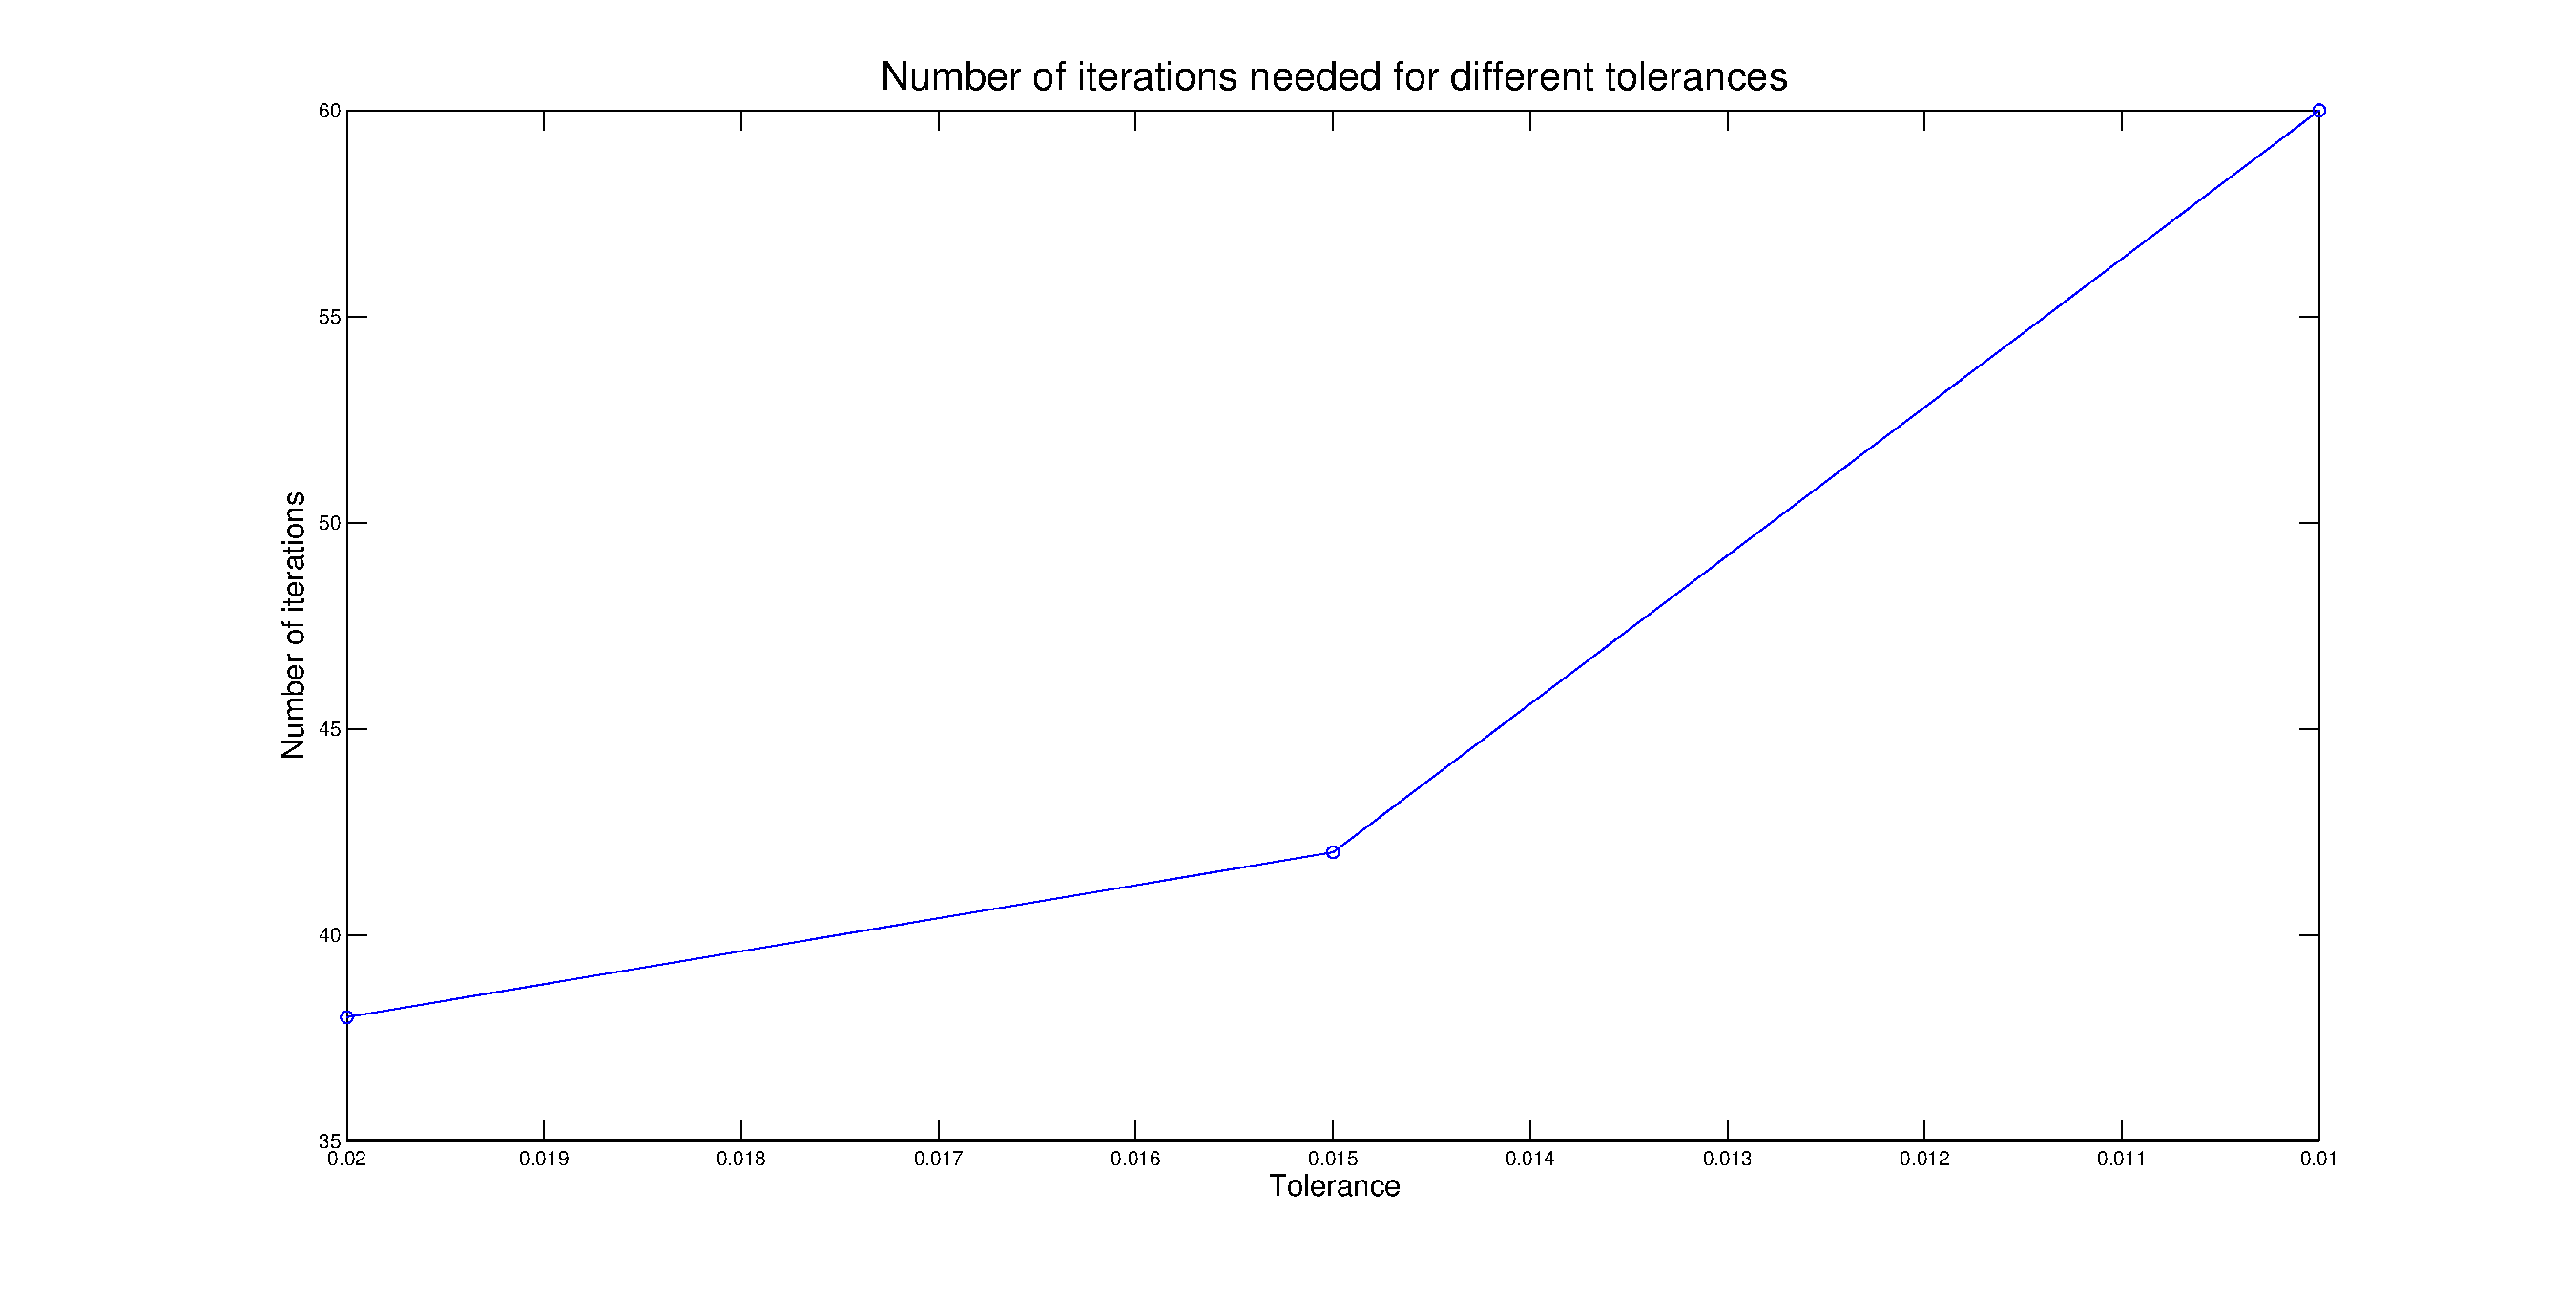
\includegraphics[scale=0.35]{Results/fine_hang_plot.eps}
\caption{Number of iterations needed to reach a given norm on the residual for a degree of interpolation $p=2$ and for meshes obtained with different tolerances.}
\label{fine_hang_plot}
\end{figure}


Let us now see how the number of iterations varies for the different meshes. Figure \ref{fine_hang_plot} shows the number of iterations needed to reach the same norm on the residual as before for the three different meshes obtained with the tolerances presented in table \ref{fine_hanging_ratio}. We can see on the graph that the number of iterations increases when we have relatively more hanging nodes. We have to be careful since this phenomenon can also be explained by the fact that we have more quadrants when the tolerance gets tighter and that also causes an increase in the number of iterations as showed earlier in this section. However, it is observed that we need less iterations when we do not have hanging nodes and for a similar number of quadrants (for example, for 1024 quadrants without hanging nodes, we need 18 iterations whereas we need 38 for 1276 quadrants). 


As explained in the theory chapter, when we have hanging nodes, we do not treat all hanging possibilities and therefore we have an error when we compute the local residual. This explains why we need more iterations in presence of hanging nodes and the fact that we converge less quickly the more hanging nodes we have in the mesh. However, the number of iterations is still acceptable.

\subsubsection{Increasing the degree of the interpolation} 

\begin{figure}
\centering
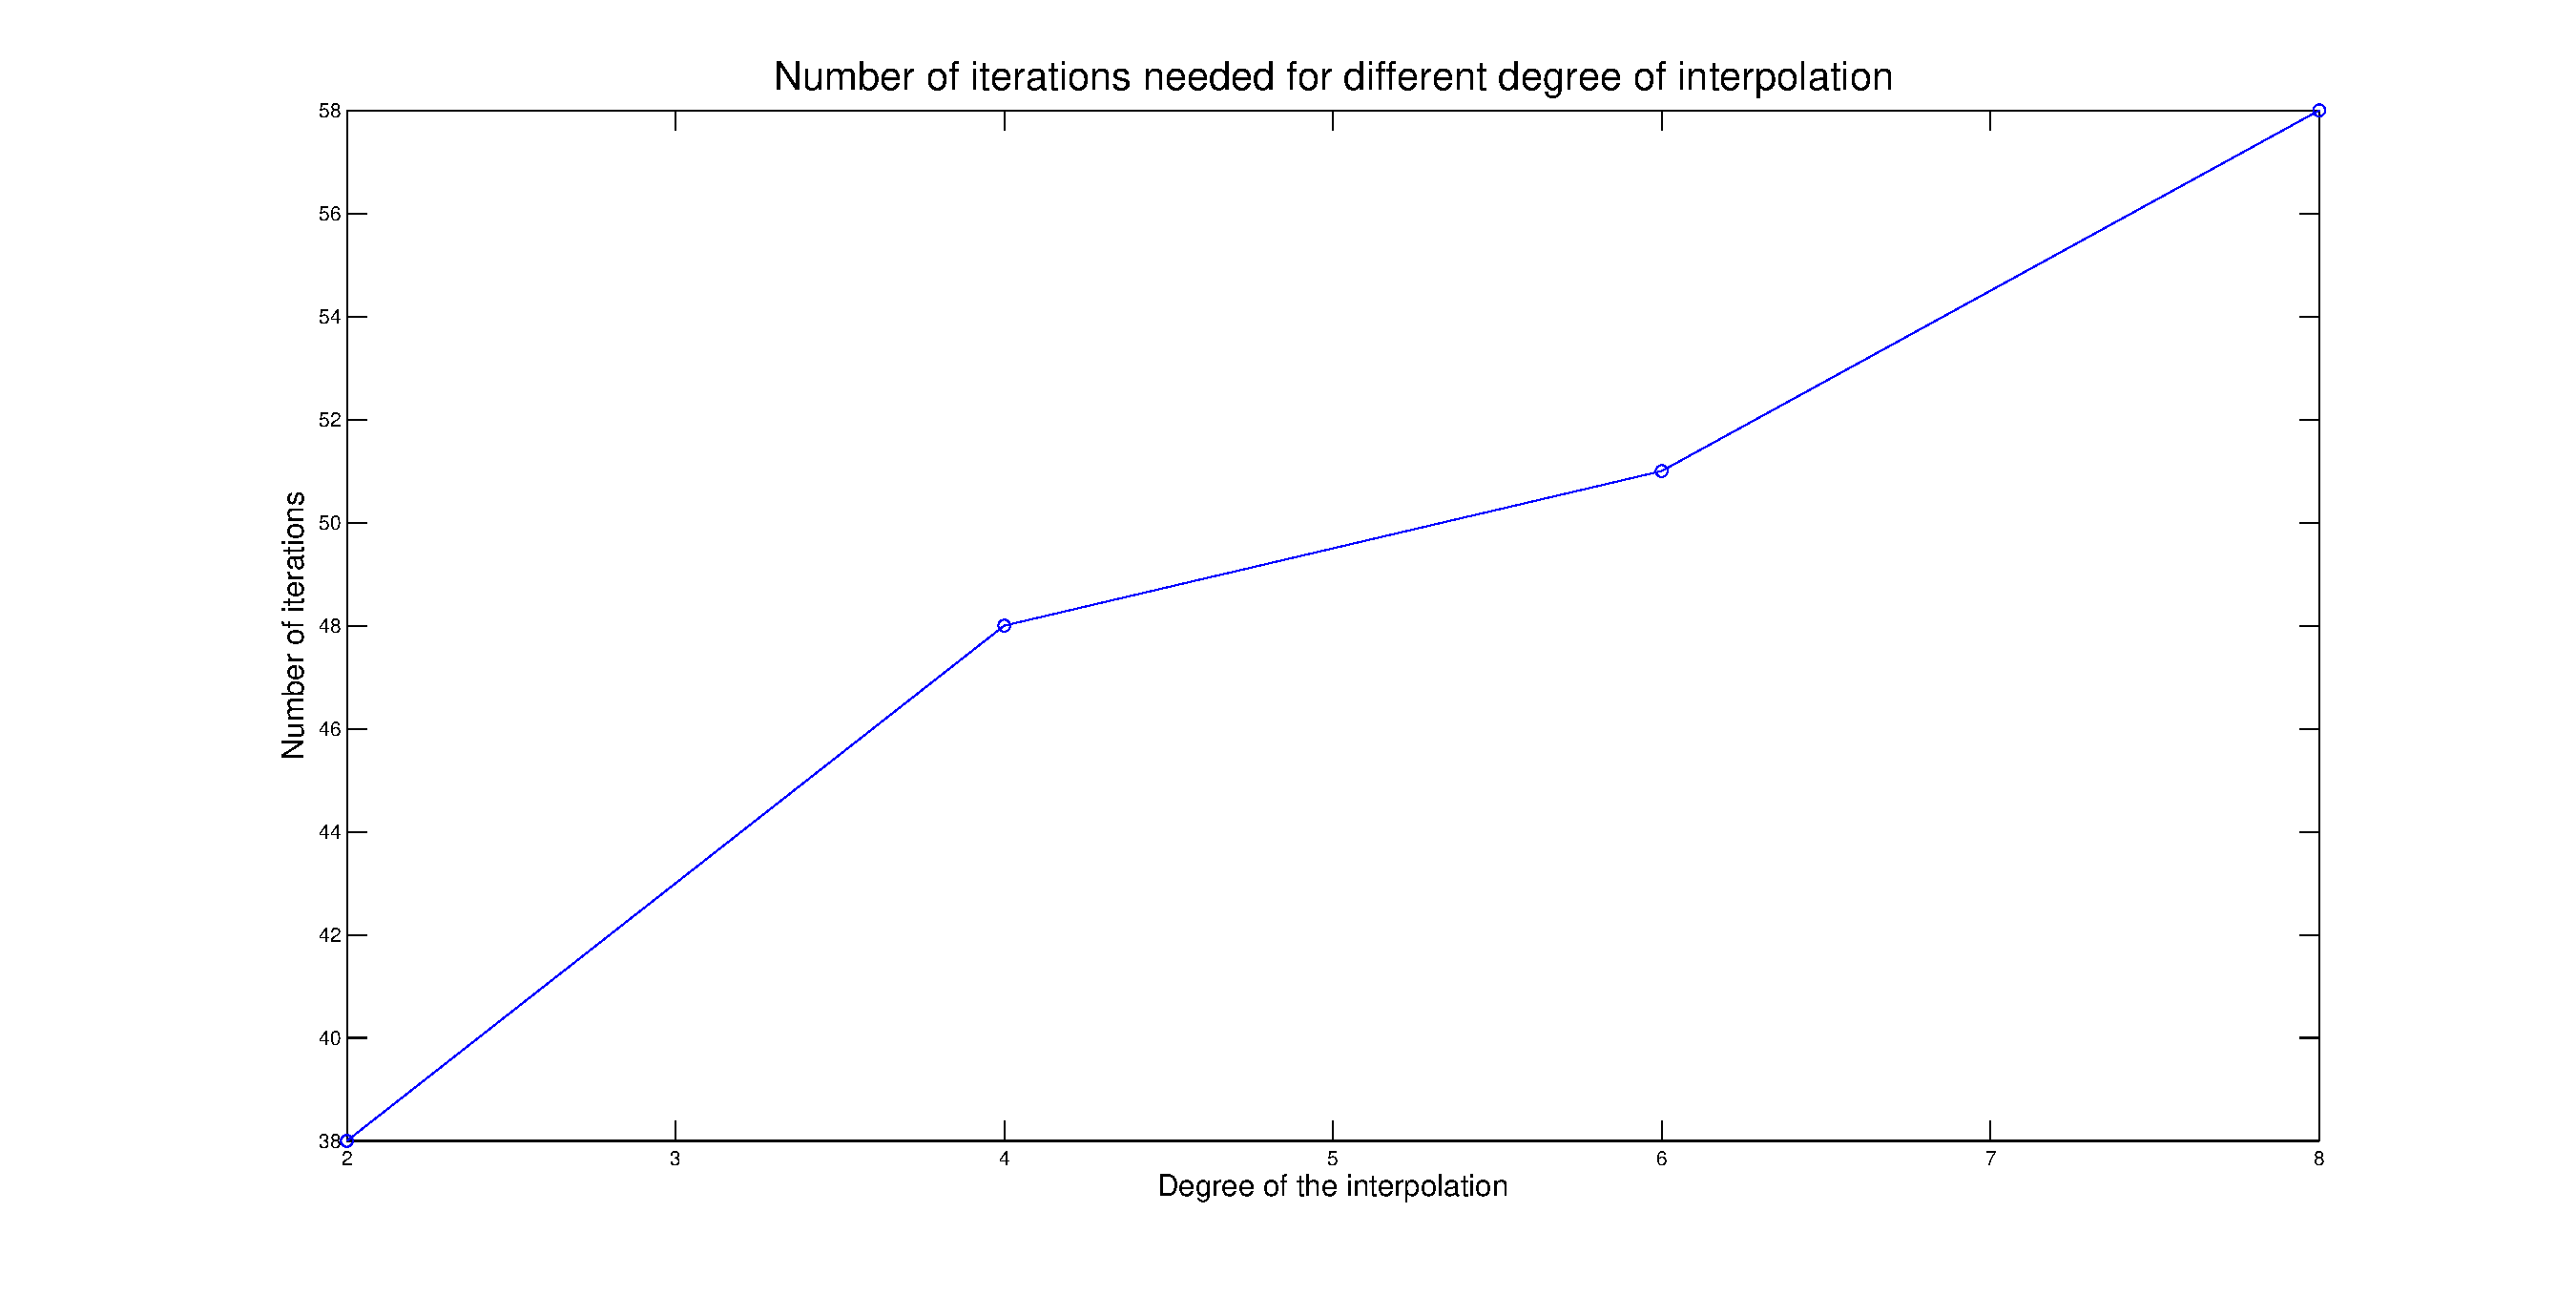
\includegraphics[scale=0.35]{Results/fine_hang_deg.eps}
\caption{Number of iterations needed to reach the tolerance of the norm of the residual as a function of the degree of the interpolation used for a mesh obtained using $tol=0.02$ in the recursive refine function.}
\label{fine_hang_deg}
\end{figure}

Let us finally look at what happens when we increase the degree of the interpolation. We tried different degrees of interpolation ($p=2,4,6,8$) and look at the number of iterations needed to obtain the numerical solution. Figure \ref{fine_hang_deg} shows the results.  

We can see that the number of iterations increases with the degree. We need 38 iterations for $p=2$ but 58 for $p=8$. As already explained in the case with no hanging nodes, this is in part due to the fact that when we increase the degree of the interpolation, the size of the overlap decreases and therefore we need more iterations.

We can also mention the fact that since we do not treat all hanging possibilities when we compute the local residual at the overlaps, increasing the degree (and therefore the number of nodes in the overlaps) might have a effect on the number of iterations.

All the tests presented here were on meshes where the elements were not distorted and where we expect the fine preconditioner to behave optimally but the same tests have been performed with distorted quadrants and we observe the same qualitative results. 


 



 

\section{Two scale preconditioner}

Let us finally move on to the two-scale preconditioner. We showed in the previous part that using only the fine scale preconditioner was not a good idea when the number of quadrants increased (the number of iterations roughly doubles when the mesh size is divided by two). As explained in the theory chapter, the idea is to add a coarse part in the preconditioner (i.e. $P = P^f + P^c$), consisting mainly of solving a problem with an interpolation degree $p=1$ with a geometric multigrid method, so that the number of iterations stays constant when we increase the number of quadrants.  

As in the previous section, the tests will be performed in two parts : first, we will analyze the performances of the two-scale preconditioner when there are no hanging nodes (but for both regular and distorted meshes) and then we will look at what happens when the forest of quadtrees is refined recursively and therefore the mesh is not conforming anymore. 

In the last subsection, we will also motivate the choice of using higher order degrees of interpolation. We will indeed look at the best degree to obtain a given accuracy in the solution, i.e. the degree for which we have the solution to a given problem on a given mesh in the shortest amount of time and that is accurate enough. 

\subsection{No hanging nodes}

Let us first present the problem we will solve in this part. We want our numerical solution to capture both low and high frequency modes so we will superpose a cosine with low frequency and a sine with a high frequency. As before, the domain is : $\Omega = \left[ -1;1 \right]^2$ and $\Gamma$ is the boundary. We will solve : 

\begin{align}
\nabla^2 u &= -\frac{\pi^2}{2}\cos(\frac{\pi}{2}x)\cos(\frac{\pi}{2}y) - 5\pi^2\sin(5\pi x)\sin(5\pi y) &\text{on $\Omega$} \label{eq:prob_two}\\
u &= 0  &\text{on $\Gamma$}
\end{align}

This problem has an analytic solution that is given by : 

$$ u(x,y) = \cos(\frac{\pi}{2}x)\cos(\frac{\pi}{2}y) + \frac{1}{10}\sin(5\pi x)\sin(5\pi y)$$

\begin{figure}
\centering
\includegraphics[scale=0.35]{Results/two_simple_sol.eps}
\caption{Numerical solution to problem \ref{eq:prob_two} using an interpolation of order $p=2$ and $1.0\:10^{6}$ degrees of freedom on a regular mesh with no hanging nodes. This numerical solution has been obtained by the PCG with the two scale preconditioner.}
\label{two_simple_sol}
\end{figure}


An example of a numerical solution obtained using the preconditioned conjugate gradients with the two scale preconditioner can be seen on figure \ref{two_simple_sol}. This solution has been obtained in only 8 iterations and with an interpolation of degree $p=2$. 

\subsubsection{Regular meshes}

Let us now look at what happens to the number of iterations when we decrease the mesh size for different degrees of interpolation. Table \ref{two_table_reg} shows the number of degrees of freedom for the different meshes used (indeed, for a given mesh, the higher the degree of the interpolation, the more global nodes we have). We can already see that, thanks to the coarse preconditioner, we are able to have a lot more degrees of freedom than in the case where we only had the fine preconditioner.

\begin{table}
\centering
\begin{tabular}{c|cccc}
\hline
Number of quadrants & $128^2$ & $256^2$ & $512^2$ & $1024^2$\\
\hline
$p=2$ & $6.6\:10^4$ & $2.6\:10^5$ & $1.1\:10^6$ & $4.2\:10^6$ \\
$p=4$ & $2.6\:10^5$ & $1.1\:10^6$ & $4.2\:10^6$ & $1.7\:10^7$ \\
$p=6$ & $5.9\:10^5$ & $2.4\:10^6$ & $9.4\:10^6$ & $3.8\:10^7$ \\
$p=8$ & $1.1\:10^6$ & $4.2\:10^6$ & $1.7\:10^7$ & $6.7\:10^7$ \\
\hline
\end{tabular}
\caption{Number of degrees of freedom for a regular mesh with different numbers of quadrants and for different degrees of interpolation.}
\label{two_table_reg}
\end{table}

\begin{figure}
\centering
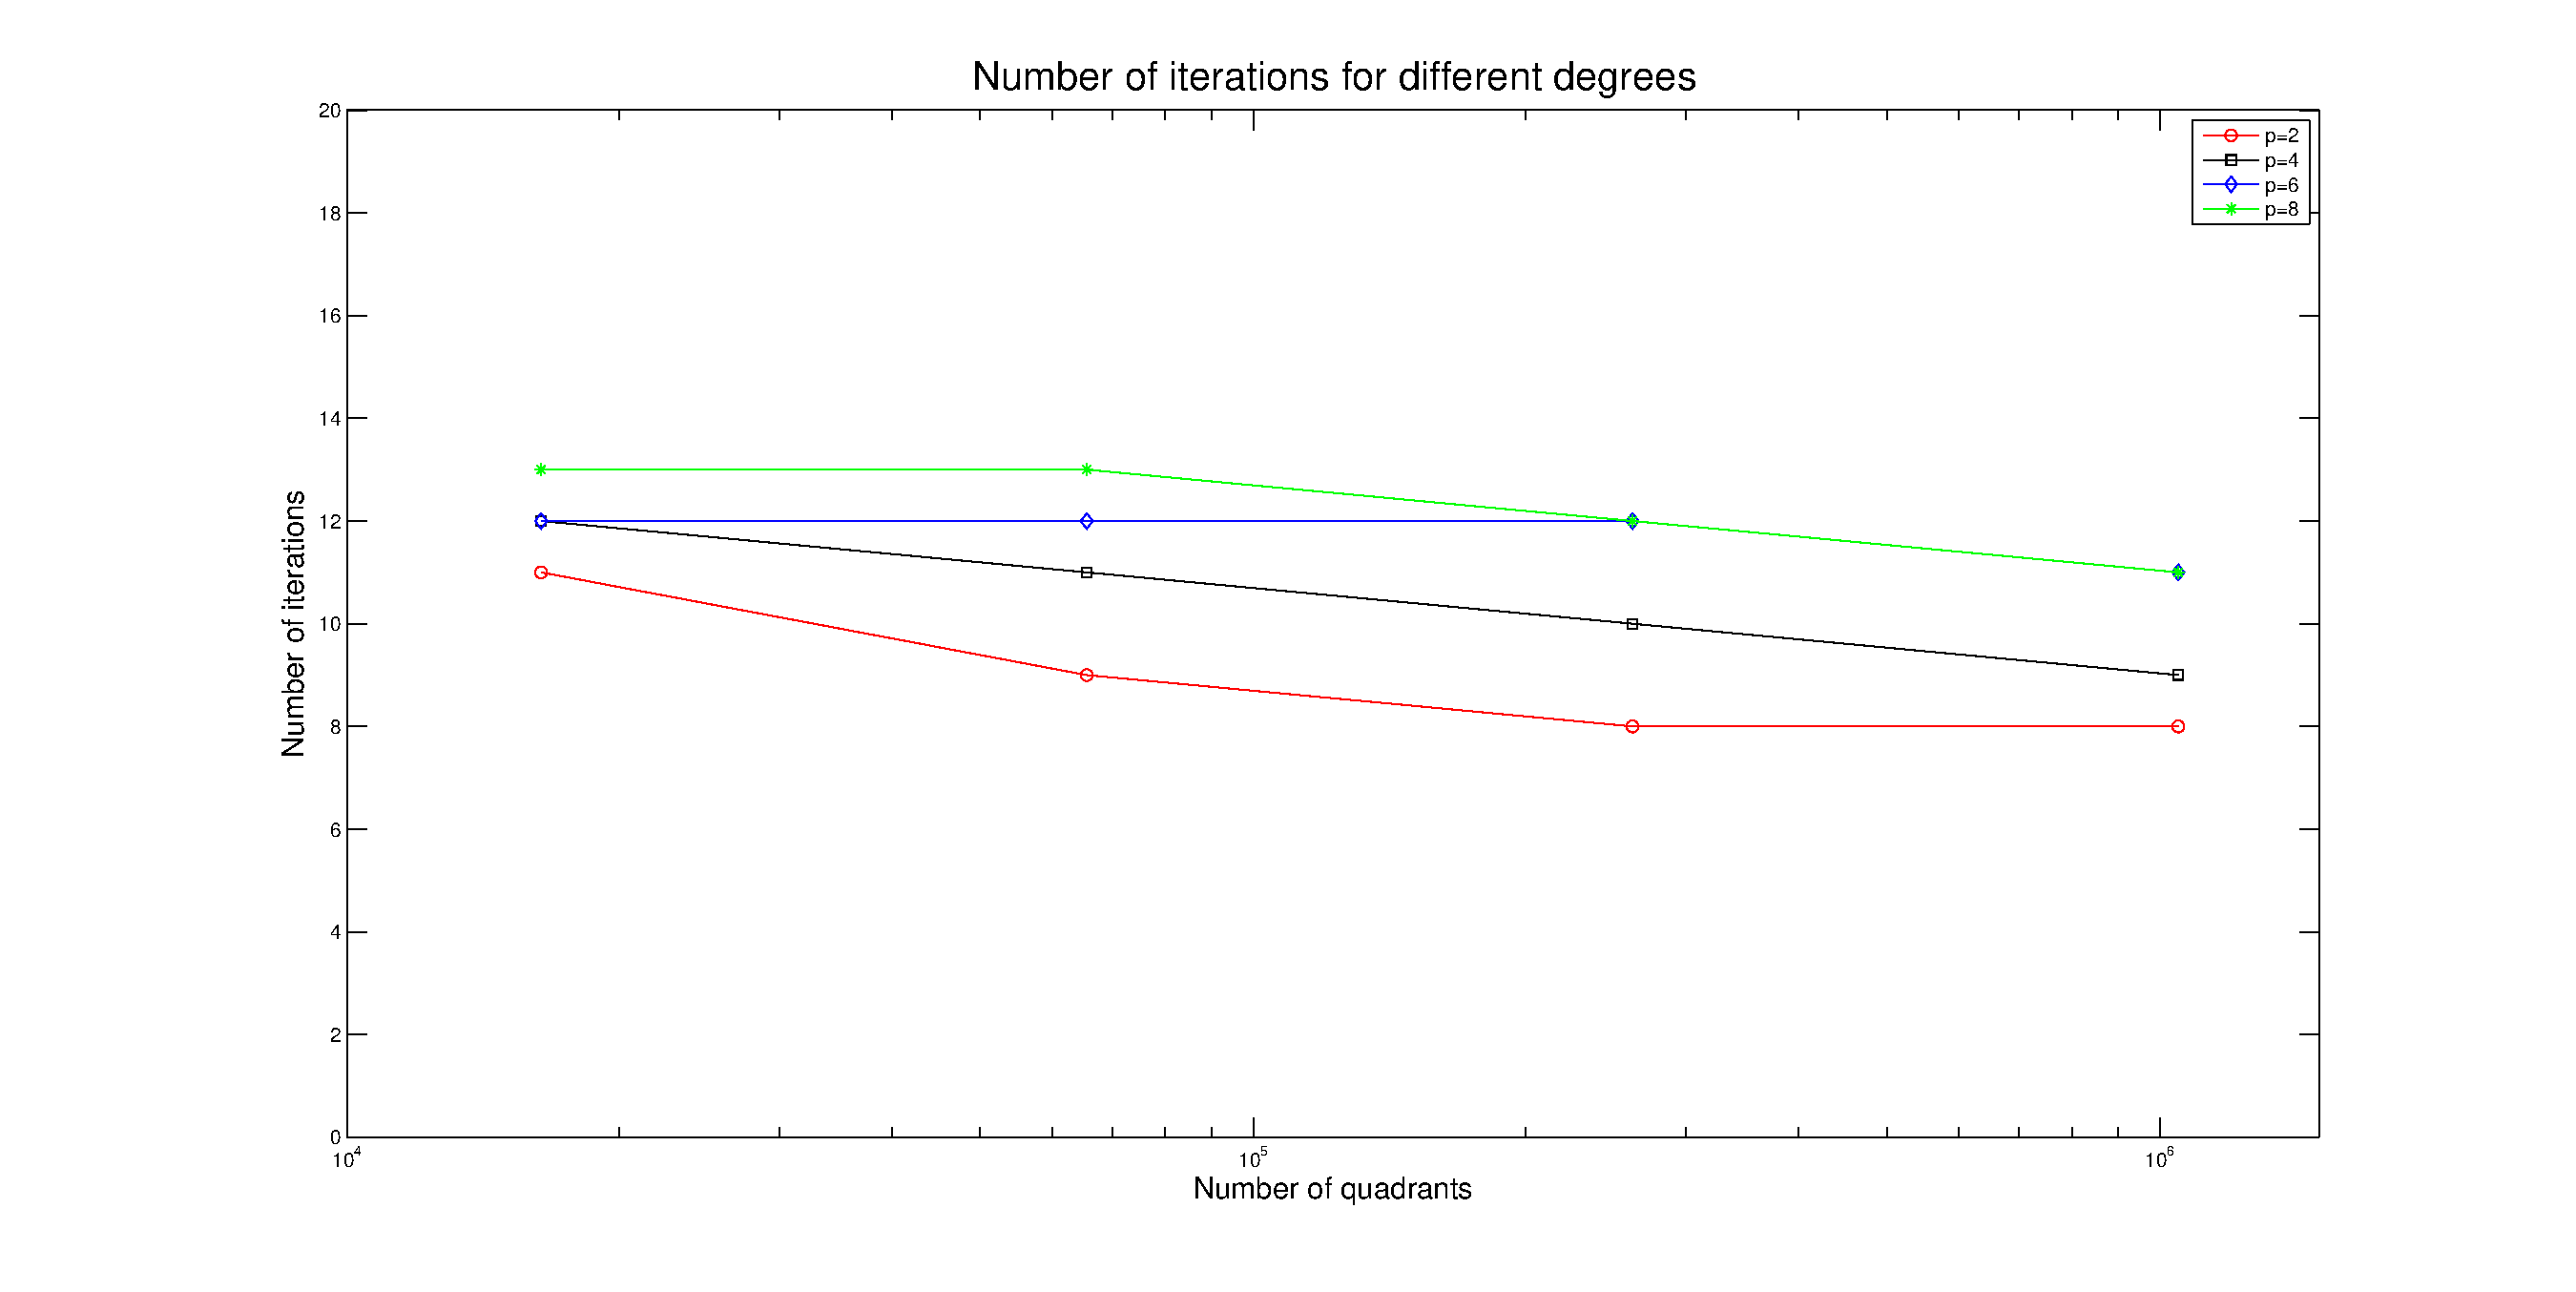
\includegraphics[scale=0.35]{Results/two_reg_iter.eps}
\caption{Number of iterations of PCG with the two scale preconditioner for degree $p$ of interpolation needed to reach the given tolerance of the norm of the residual as a function of the number of quadrants in a regular mesh.}
\label{two_reg_iter}
\end{figure}

For the following tests, we also have tighten the tolerance on the norm of the residual. We now require that : 

$$\frac{||r_k||_2}{||r_0||_2} < 10^{-5}$$

Figure \ref{two_reg_iter} shows the number of iterations needed to reach that tolerance of the norm of the residual when we use our two scale preconditioner for different degrees of interpolation. The first remark we can make is that the number of iterations does not increase with the number of quadrants (as it was the case when we only had the fine preconditioner). So we can conclude that the coarse preconditioner does the job it was designed to do. We can even note that the number of iterations slightly decreases. For example, for $p=6$, we need 12 iterations for $128^2$ quadrants but we only do 11 iterations for $1024^2$. An explanation for this phenomenon might be that when we increase the number of quadrants, we actually better separate the actions of the fine and coarse preconditioners and therefore the sum of the two is a better approximation of $A^{-1}$. We can mention that for $p=8$, we only need 11 iterations to solve a system that has more than 67 millions unknowns. 

A second remark we can make, as already observed when we only had the fine preconditioner, is that the number of iterations grows with the degree of the interpolation. For example, with $1024^2$ quadrants, we need 8 iterations when $p=2$ but we need to do 11 iterations when $p=8$. As before, this can be explained by the fact that as the degree of the interpolation increases, the size of the overlap decreases. A fixed sized overlap would fix this issue. 

\subsubsection{Meshes with distorted elements}

We will now look at what happens when the mesh is not regular but we have quadrants that are more and more distorted. We will use the same meshes already used in the previous section and obtained with the progression tool of GMSH (see figure \ref{fine_mesh_deform} for example of such meshes).

\begin{figure}
\centering
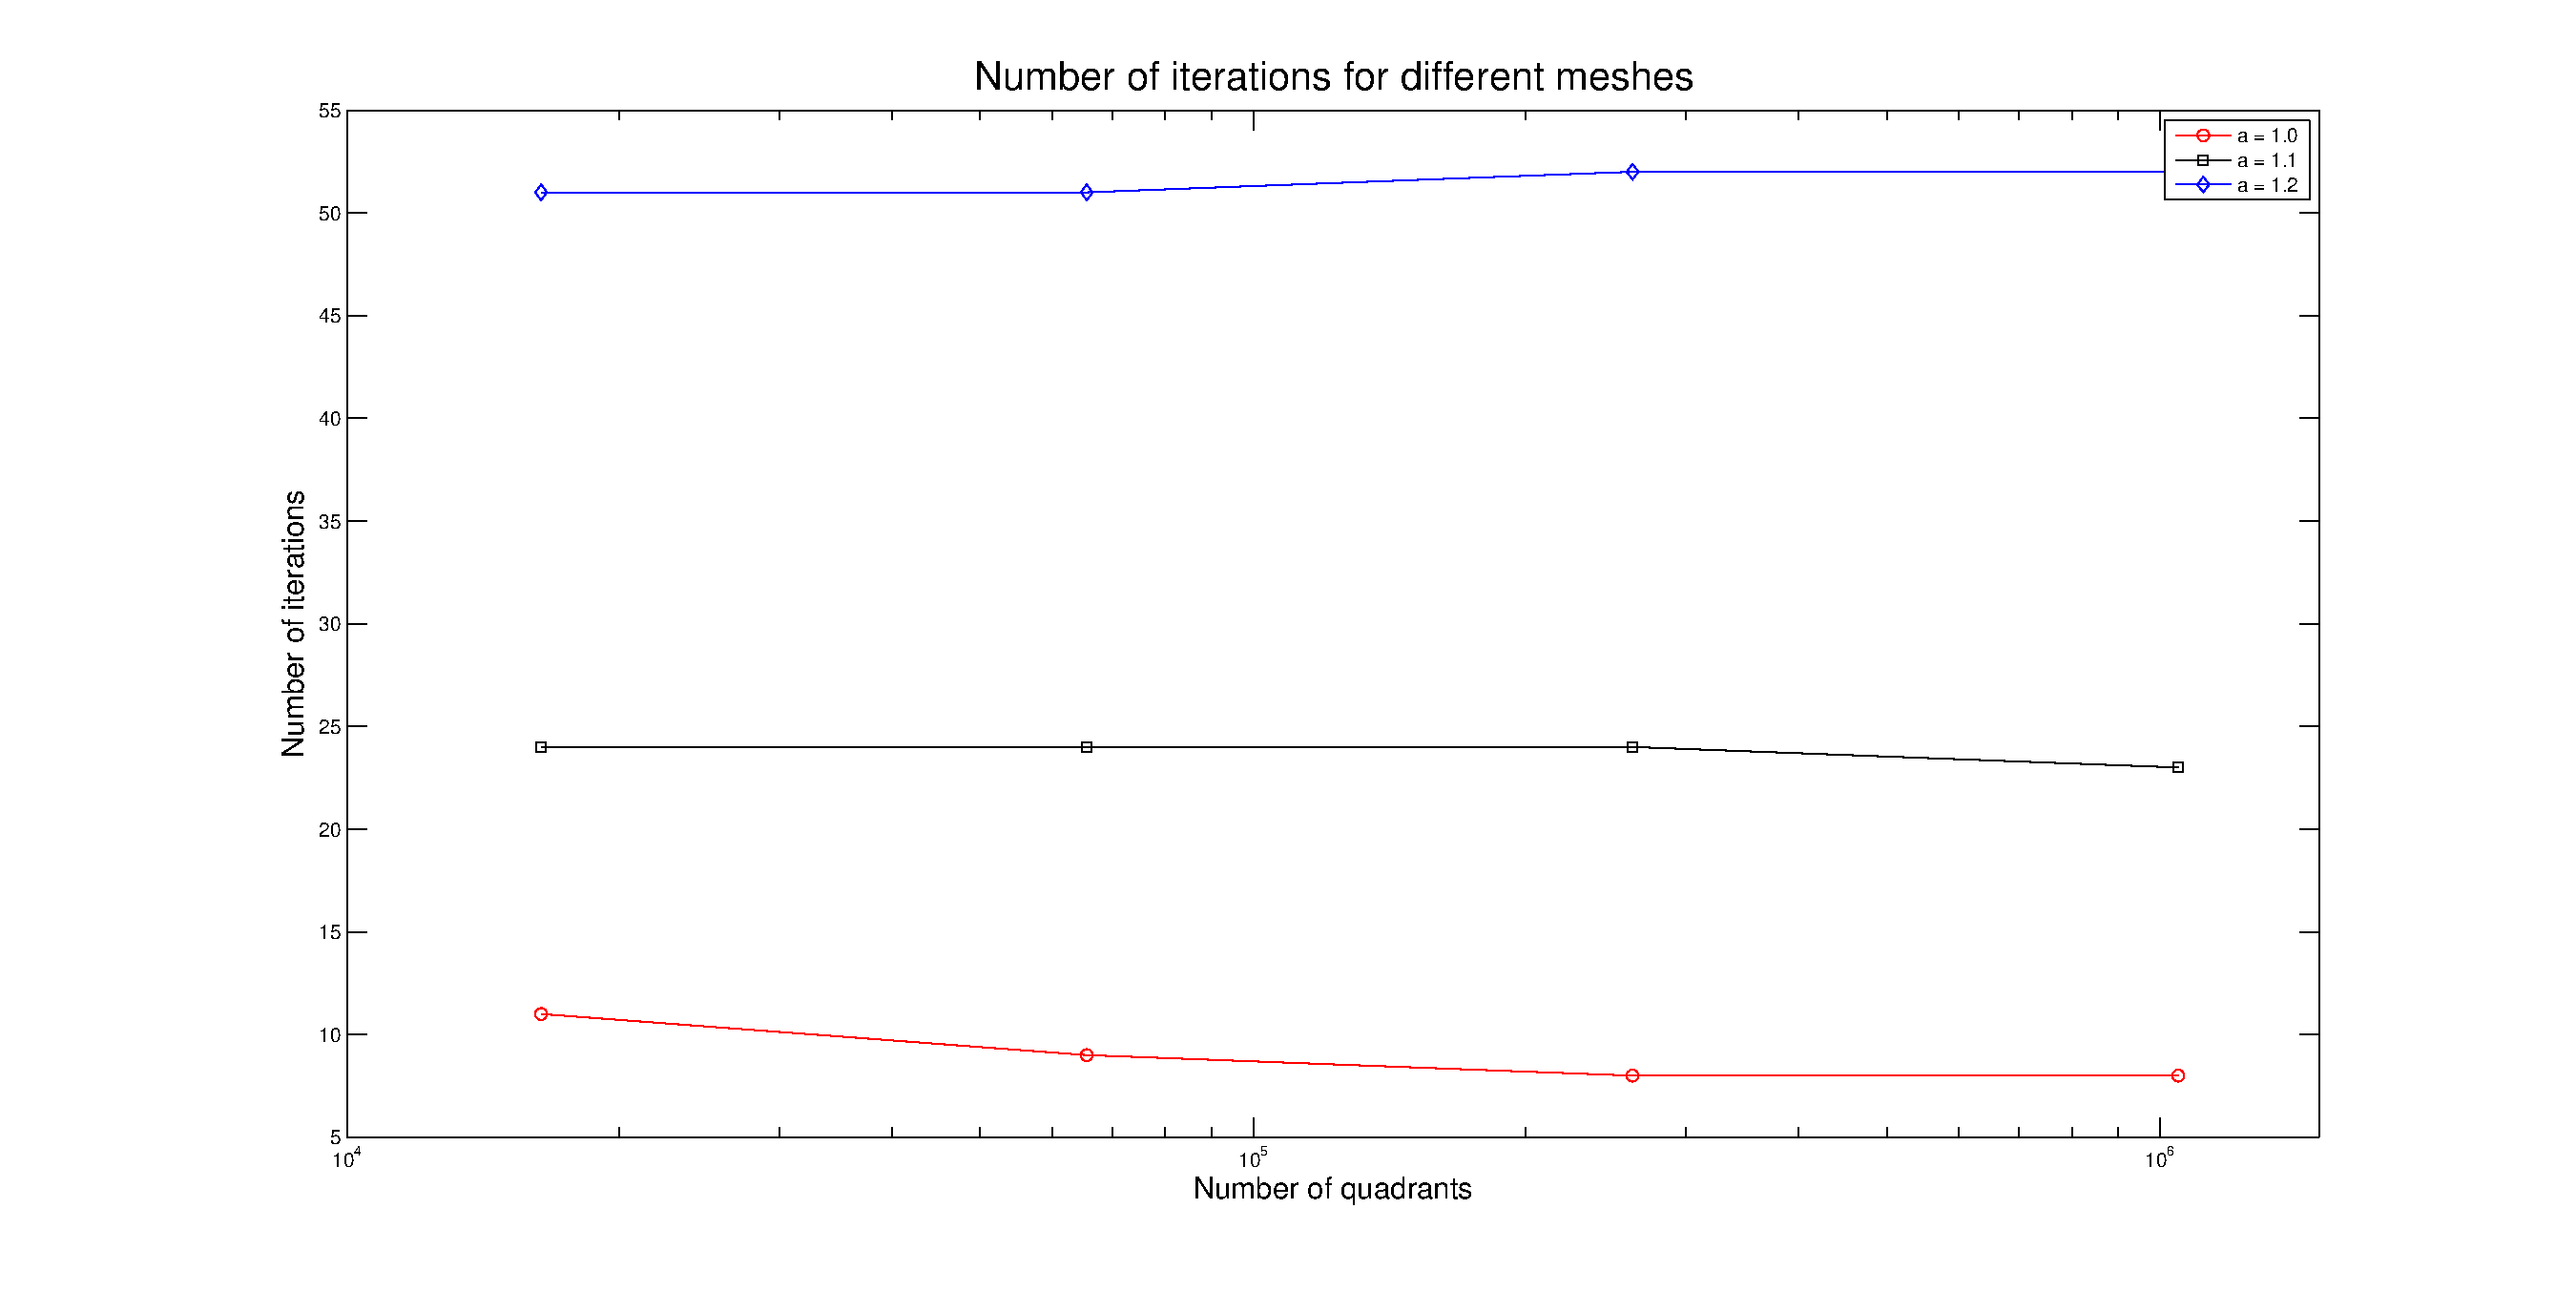
\includegraphics[scale=0.35]{Results/two_irreg_iter.eps}
\caption{Number of iterations of PCG with the two scale preconditioner for an interpolation degree $p=2$ needed to reach the given tolerance on the norm of the residual as a function of the number of quadrants for meshes with quadrants more and more distorted.}
\label{two_irreg_iter}
\end{figure}

For an interpolation of degree $p=2$, we looked at the number of iterations needed to reach the given tolerance as we increased the number of quadrants and for elements more and more distorted. Figure \ref{two_irreg_iter} shows the results. We can see that the number of iterations stays roughly the same when we increase the number of quadrants so once again the coarse part of the preconditioner does the job it is designed to do. 

We can also node that the more we distort the quadrants the more iterations we need to reach the given tolerance. This is to be expected since we developed the fine preconditioner to work optimally on quadrants aligned with the axis. This means that the more a quadrant is distorted the less accurate is the fine preconditioner part and therefore the more iterations we need. However, even with the most distorted mesh, the number of iterations stays acceptable and as explained in the previous section, the gain of not having to solve exactly on every quadrant is huge. We also have to say that the meshes presented here have an intrinsic structure since they are generated using the progression tool in GMSH. Therefore, the errors we make with our approximation are always in the same direction and the number of iterations needed increases. We might not have such an increase with a random mesh containing quadrants with the same quality measure. 


\subsection{Influence of hanging nodes}

Let us now move on to the cases where we have hanging nodes. As in the part with only the fine preconditioner, we will look at a problem where the solution has a jump so that we create hanging nodes when we use a recursive refine function in p4est. In addition to the hyperbolic tangent already presented in the previous subsection, we will include a high frequency sine wave to see how the grid adapts to capture it and how the two scale preconditioner performs in its presence. 

The problem we will solve is : 

\begin{align}
\nabla^2 u =& -2\tanh(12x)\tanh(12y)\left[ 12^2(1-\tanh(12x)^2) + 12^2(1-\tanh(12y)^2)\right] \nonumber \\
 &-  10\pi^2\sin(10\pi x)\sin(10\pi y) &\text{on $\Omega$} \label{eq:two_hang}\\
u =&   \tanh(12x)\tanh(12y) + \frac{1}{20}\sin(10\pi x)\sin(10\pi y)&\text{on $\Gamma$}
\end{align}

Where $\Omega = [-1;1]^2$ and $\Gamma$ is the boundary. This problem has an analytic solution that is given by : 

$$u(x,y) = \tanh(12x)\tanh(12y) + \frac{1}{20}\sin(10\pi x)\sin(10\pi y)$$

\begin{figure}
\centering
\includegraphics[scale=0.35]{Results/two_hang_plot.eps}
\caption{Numerical solution to problem \ref{eq:two_hang} using an interpolation of order $p=2$ on a non conforming mesh and obtained with PCG with the two scale preconditioner.}
\label{two_hang_plot}
\end{figure}

Figure \ref{two_hang_plot} shows an example of the numerical solution computed on a non conforming mesh with PCG and the two scale preconditioner. We can see on the plot both the steep jump due to the hyperbolic tangent and the small oscillations due to the sine wave.

\subsubsection{Increasing the relative number of hanging nodes}

Let us now look at the influence of increasing the number of hanging nodes in the mesh. To achieve this, we will use the same rule in the recursive refinement of the quadrants as in the previous section, given by relation \ref{hang_rel}. We will also tighten the parameter $tol$ used in order to have more quadrants than in the case when we only had the fine preconditioner. 

\begin{table}
\centering
\begin{tabular}{c|ccccccc}
Parameter $tol$ & 0.01 & 0.008 & 0.006 & 0.004 & 0.002 & 0.001 & 0.0005\\
\hline
Number of hanging nodes & 6080 & 8064 & 11008 & 14272 & 23200 & 33696 & 70112\\
Number of global nodes & 19921 & 25545 & 32265 & 49265 & 120201 & 208137 & 445425\\
$hang$ & 30.52\% & 31.57\% & 34.12\% & 28.97\% & 19.30\% & 16.19\% & 15.74\%
\end{tabular}
\caption{Statistics about the different meshes used for the tests regarding the influence of hanging nodes on the number of iterations as well as the ratio $hang$ defined by equation \ref{hang_frac}. The number of global and hanging nodes are for an interpolation degree $p=2$.}
\label{two_hang_table}
\end{table}

Table \ref{two_hang_table} shows some statistics about the different meshes used for the tests regarding the influence of hanging nodes on the number of iterations. The number of global and hanging nodes are for an interpolation of degree $p=2$ and the ratio $hang$ is given in equation \ref{hang_frac}.

We can see that, as expected, when we decrease the parameter $tol$, we have more hanging nodes. We can also see that, at first, tightening the parameter $tol$ increase the ratio $hang$ and we have more hanging nodes relatively to global nodes. Then, however, even tough the number of hanging nodes still grows, the number of global nodes grows faster and therefore the ratio $hang$ decreases. This can be explained by the fact that if the parameter $tol$ is very low then we start to refine all part more equally (even the ones where the function does not vary a lot) and the relative number of hanging nodes drops. 

\begin{figure}
\centering
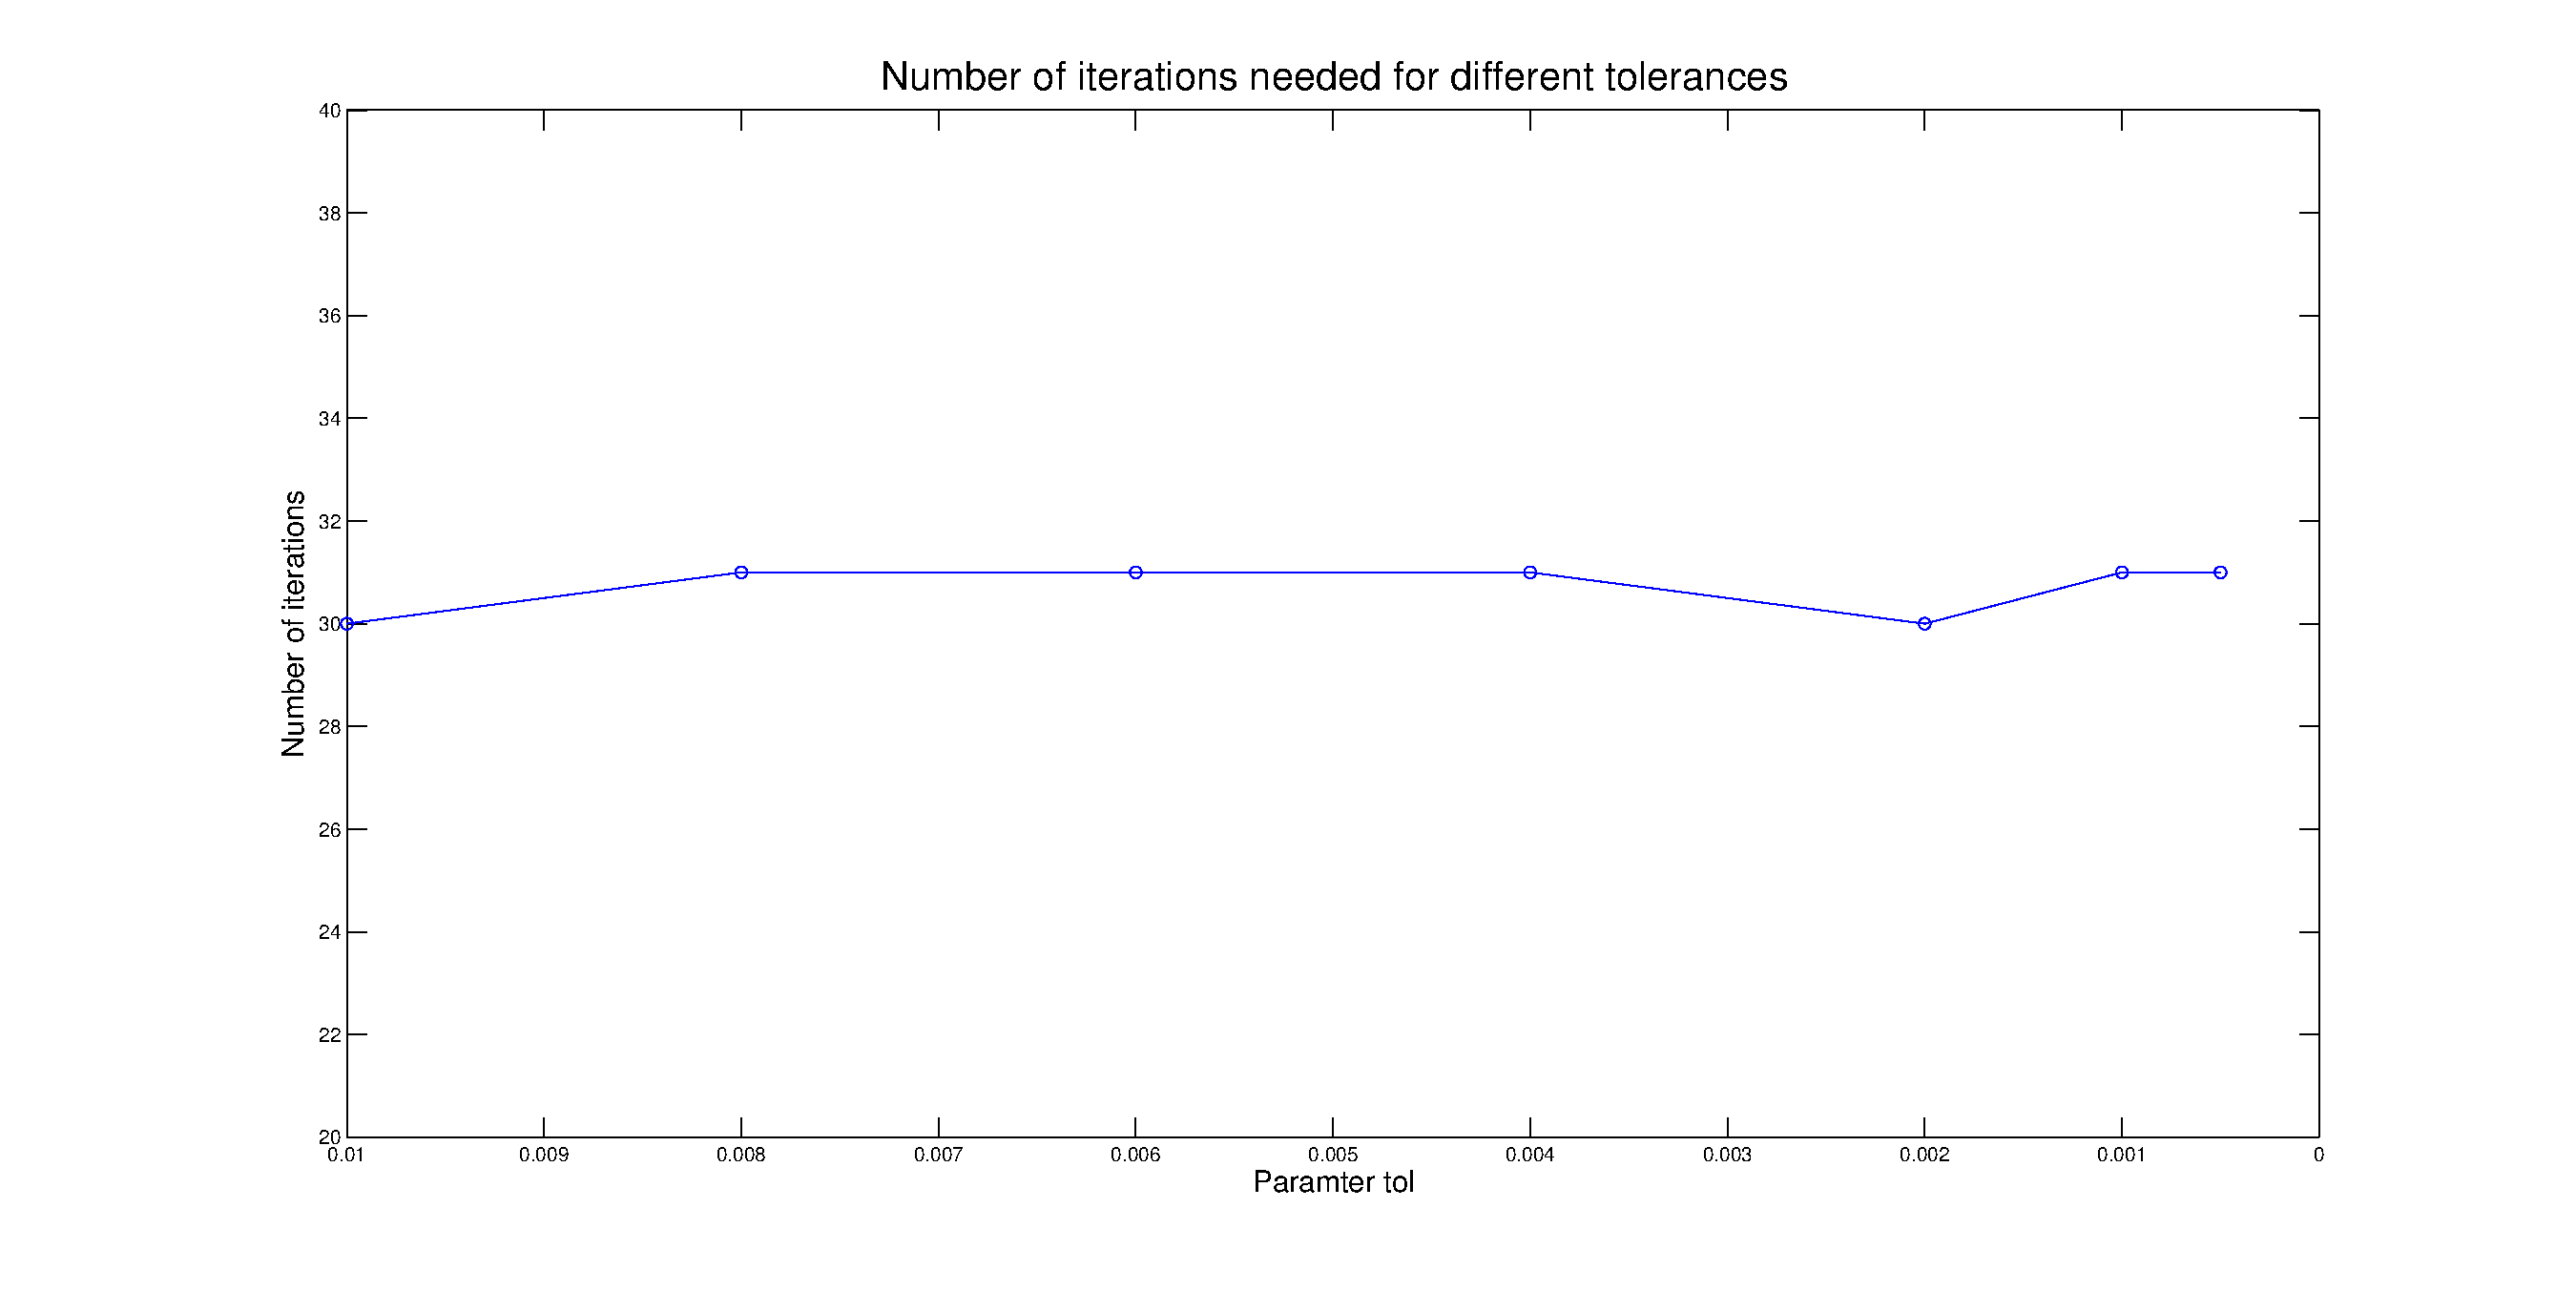
\includegraphics[scale=0.35]{Results/two_hang_iter.eps}
\caption{Number of iterations of PCG with the two scale preconditioner with a degree of interpolation $p=2$ on meshes with hanging nodes defined by the parameter $tol$.}
\label{two_hang_iter}
\end{figure}


Figure \ref{two_hang_iter} shows the number of iterations needed to reach the given tolerance with an interpolation degree $p=2$ on the different meshes presented in table \ref{two_hang_table}. We can see that the number of iterations stays roughly the same (it is either 30 or 31) for all meshes, whatever the number of hanging nodes and the value of the ratio $hang$. So we can conclude that the coarse preconditioner once again guaranties the h-independent convergence and that the number of hanging nodes does not have a great influence on the number of iterations. 

We also have to note that, for the same problem, if we use a conforming mesh, the number of iterations needed drops to 16. So even if the number of hanging nodes (absolute or relative) does not greatly influence the number of iterations, just adding one non conforming quadrant does a lot to decrease the performance of the preconditioner. We can point the fact that, as mentioned earlier, when we have hanging quadrants, we do not handle every possibilities to compute the residuals in the overlaps. We can thus see how that affects the number of iterations. 


\subsubsection{Increasing the degree of the interpolation}

\begin{figure}
\centering
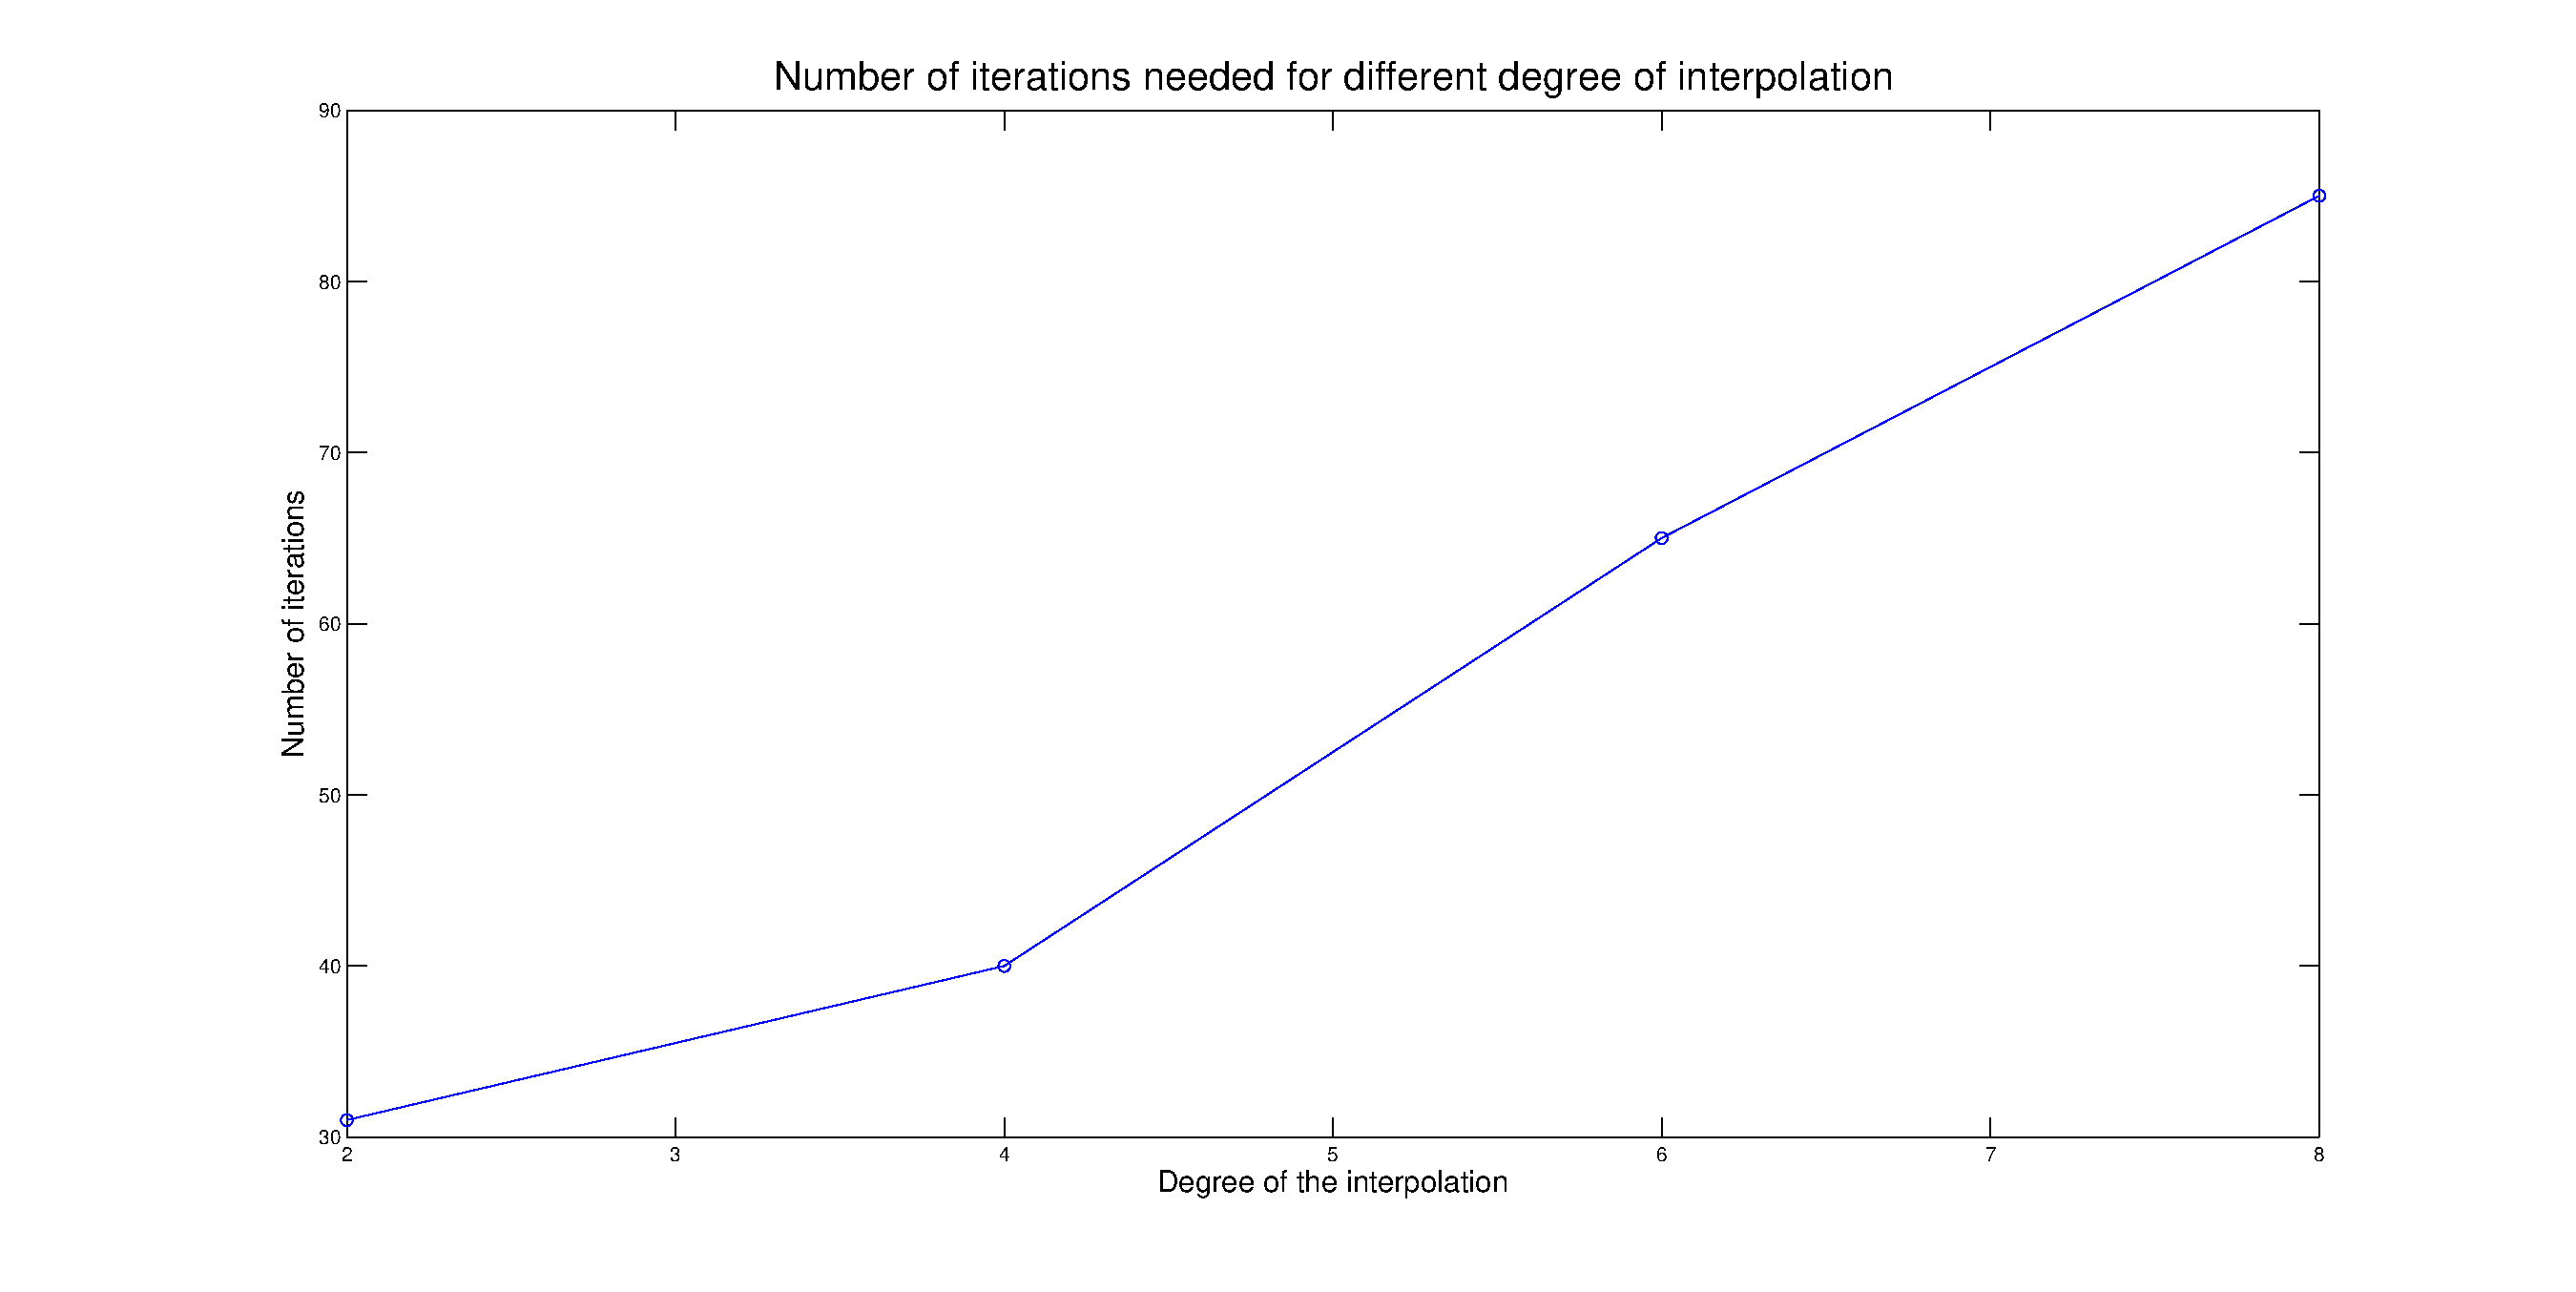
\includegraphics[scale=0.35]{Results/two_hang_deg.eps}
\caption{Number of iterations of PCG with the two scale preconditioner as a function of the degree of the interpolation used for a mesh obtained with $tol = 0.001$ in the recursive refine function.}
\label{two_hang_deg}
\end{figure}

Let us now move on to look at what happens when we increase the degree of the interpolation. We will use the mesh defined by $tol = 0.001$ and look at the number of iterations needed to reach the given tolerance for $p=2,4,6,8$. Figure \ref{two_hang_deg} shows the results. 

We can see that as we increase the degree of the interpolation, the number of iterations increases. It goes from 31 for $p=2$ to 85 iterations when $p=8$. We can see that it is quite a lot. But we also have to note that going from degree 2 to degree 8, we have also gone from $2.1\:10^5$ degrees of freedom to $3.4\:10^6$.

As in the case when we only had the fine preconditioner, several factors can be put forward to explain the increase in the number of iterations. First, when we increase the degree, the size of the overlap decreases and therefore the fine preconditioner is less effective. As mentioned in \cite{overlap_constant}, a fixed sized overlap would fix the issue. 

Second, we can say that the number of hanging nodes in the overlaps increases with the degree of the interpolation. Since we do not treat all possibilities when handling hanging quadrants, the error made is more important when we have a lot of nodes in the overlaps.


\subsection{Most efficient degree to obtain a given accuracy}

In this subsection, we will look at the best degree of interpolation $p$ to obtain a given accuracy. We will use the problem defined by \ref{eq:prob_two} and the distorted mesh using the progression tool of GMSH with $a=1.2$ that we will uniformly refine. We will also tighten the tolerance on the norm of the residual since we want the error to come from the interpolation and not from the fact that we only solve the linear system approximately. We will impose that : 

$$ \frac{||r_k||_2}{||r_0||_2} < 10^{-12} $$

Afterwards, we will compute the error committed by the discretization in the $L^2$-norm. Let us define $e^p$, the error made by using an interpolation of degree $p$, $u^p$ the solution of the discretized problem using a degree $p$, $U^p_i$ the numerical solution at the global node $i$ of the linear system that arises and $m_i$ the mass matrix associated with the integration. Then we have :  

\begin{align}
e^p &= \left( \int_\Omega (u-u^p)^2dxdy \right)^\frac{1}{2}\\
 &\approx \left( \sum_i (u(x_i,y_i)-U_i^p)^2 m_i \right)^\frac{1}{2}
\end{align}

We can note that if we refine uniformly the mesh, then $e^p$ will decrease but it will also cost us more. And for a given mesh, we have that $e^p$ decreases as $p$ increases (but it also costs us to increase the degree). So the question that arises is when is it more interesting to refine the mesh uniformly and when is it better to increase the degree of the interpolation to get the accuracy we want.

We will select degree $p$ to be the best for an accuracy of $10^{-a}$ if and only if there is a mesh such that $e^p<10^{-a}$ on this mesh and the time needed to obtain the numerical solution is smaller than for any degree on any other mesh and the same accuracy. 

\begin{figure}
\centering
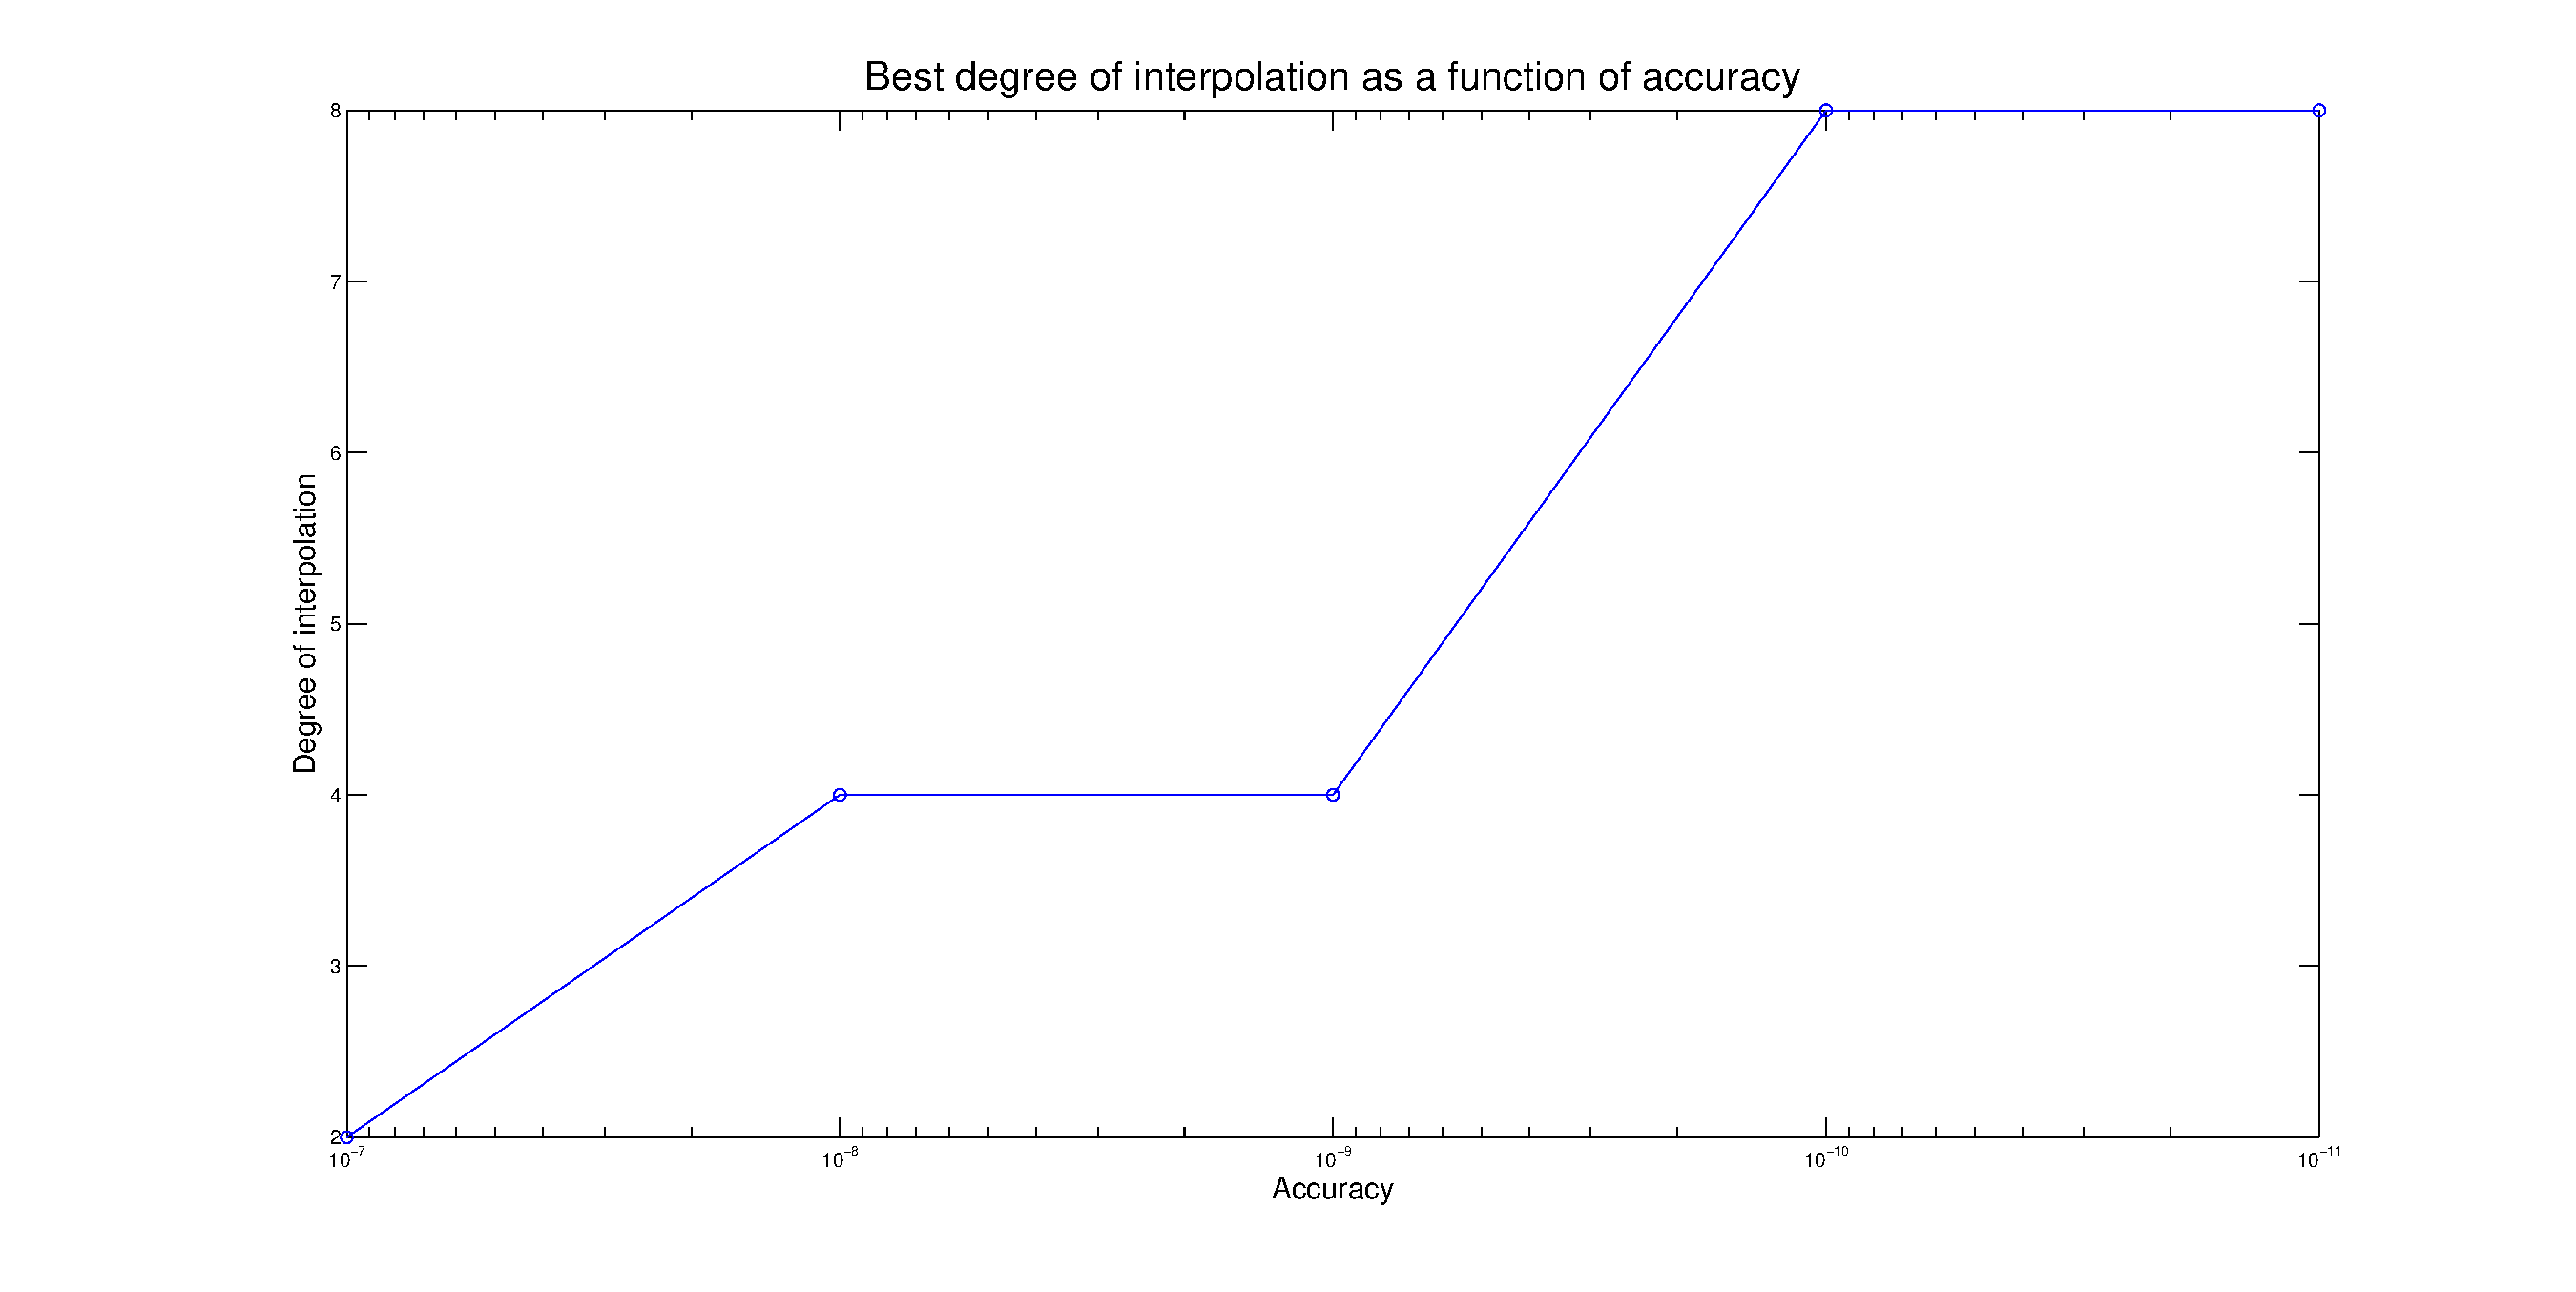
\includegraphics[scale=0.35]{Results/two_acc.eps}
\caption{Best degree of interpolation to solve problem \ref{eq:prob_two} on a distorted mesh as a function of the accuracy we want on the $L^2$-norm.}
\label{two_acc}
\end{figure}

Figure \ref{two_acc} shows the results. We can see that when the wanted accuracy is rather low (for $10^{-7}$) then it is quicker to use an order of interpolation $p=2$ because the number of iterations needed to solve the linear system is smaller than for a higher order interpolation. Moreover, the number of degrees of freedom to obtain such an accuracy is not so high as to make one iteration very long. 

On the other hand, when we want a better accuracy ($10^{-10}$, $10^{-11}$) then it is cheaper to use higher order interpolation such as $p=8$. This can be explained by the fact that, even though the number of iterations of PCG is higher (as mentioned earlier in this section), the number of degrees of freedom to obtain the wanted accuracy is much lower for $p=8$ than for the other degrees. Therefore, one iteration takes much less time and $p=8$ becomes more efficient. 

In between the two ($10^{-8}$, $10^{-9}$), we can see that the best degree is $p=4$ where we have a trade-off between the number of iterations needed to solve the system and the number of degrees of freedom.

The quantitative results presented here depend of course of the implementation, the problem to solve and the mesh used. However, we can note that the qualitative result stays true : the more accurate we want to be, the more interesting it becomes to use higher degree in the interpolation because then the number of DOF does not grow as large as it would with lower order polynomials. 





\section{Conclusion}

Let us now summarize the results given in this chapter. 

We first looked at the properties of our geometric multigrid solver. The key property of h-independent convergence has been observed for a large variety of parameters $\nu_1$ and $\nu_2$ and various meshes that were regular or distorted. The presence of hanging nodes has no influence whatsoever on the convergence of the geometric multigrid method. 

We then moved on to the PCG with only the fine scale preconditioner. Several observations were made. We saw that, even on a regular mesh where the preconditioner is optimal, increasing the number of quadrants increased the number of iterations needed. That was predicted since increasing the number of quadrants decreases the mesh size. We also noticed that we needed more iterations when the degree of interpolation $p$ grew. That was explained by the fact that the size of the overlap diminishes when $p$ increases. We then moved on to meshes with distorted quadrants and saw that we needed more iterations than in the regular case. It was to be expected since the fine preconditioner was designed to work best on quadrants aligned with the axes. Afterwards, we introduced non conforming meshes. The presence of hanging nodes also increased the number of iterations. That was explained by the fact that we do not restrict the residual exactly in the overlaps. When we increase the degree of the interpolation on a non conforming mesh, the number of iterations increases as in the conforming case. 

The coarse grid correction was then added in the preconditioner. We first tested the PCG with the two scale preconditioner on conforming meshes and saw that we obtained the h-independence thanks to the coarse preconditioner : the number of iterations stayed constant whatever the number of quadrants and the mesh size. That was true for both meshes with regular quadrants and meshes with distorted quadrants. We can however note that the number of iterations needed was greater in the case of distorted quadrants. Again, this was to be expected since the fine preconditioner works better on quadrants aligned with the axes. We then experimented on non conforming meshes. We saw that changing the absolute or the relative number of hanging nodes in the mesh had no real impact of the number of iterations. That being said, we saw that we needed more iterations when we had hanging nodes (even a few) than when we had none. We also looked at what happened when we increased the degree of the interpolation. As before, it increases with the degree $p$. The same remarks as before also apply here. 

Finally, we picked a problem and a mesh and looked at the best degree of interpolation to solve this problem, i.e. the degree which allowed us to get the solution within a given tolerance in the $L^2$-norm the quickest. We saw that at first, for a low tolerance, a low degree is best since then the fine preconditioner is cheap to compute and we can have a lot of degrees of freedom. The number if iterations of PCG is also lower for lower degrees. Then, as we tighten the tolerance, it becomes more and more attractive to use higher degrees since they allow us to keep the number of degrees of freedom down and still get a good enough approximation to be within the tolerance. The increase in the number of iteration for higher degrees is compensated by the fact that we have a lot less degrees of freedom. This means that for a given tolerance, we have a trade-off between the number of iterations of PCG and the number of degrees of freedom.  



% Bibliography
\newpage
%\bibliographystyle{unsrt}
\bibliography{sample} 


% Back cover page
\backcoverpage

\end{document}
